\RequirePackage[ngerman=ngerman-x-latest]{hyphsubst}
\documentclass[english,ngerman]{tudscrreprt}
\usepackage{babel}
\usepackage{selinput}
\SelectInputMappings{adieresis={ä},germandbls={ß}}
\usepackage[T1]{fontenc}
\usepackage{fixltx2e}
\usepackage{scrhack}
\usepackage{tudscrsupervisor}
\usepackage{xcolor}
\usepackage{gensymb}

%%%
% Glossar
%
\AfterPackage*{hyperref}{%
	\usepackage[%
		automake,% Alphabetische Sortierung, da xindy aktiv, kein makeindex benötigt
		% mit Tex Live einfach verwendbar
		xindy={language=german-din}, % Alphabetische Sortierung nach UTF-8 und Duden oder DIN.
		acronym,% Abkürzungen
		symbols,% Formelzeichen
		%nomain,% kein Glossar
		translate=babel,% Überschriften der Glossare in der Dokumentsprache gesetzt
		nogroupskip,% automatischer Abstand zwischen den Einträgen zur Gruppierung innerhalb eines Glossars entfernen
		toc,% fügt die Verzeichnisse dem Inhaltsverzeichnis hinzu
		section=chapter,% bestimmt die Gliederungsebene der Überschrift
	]{glossaries}
	\makeglossaries
	
\newglossarystyle{acrotabu}{%
	\renewenvironment{theglossary}{%
		\begin{tabu}spread 0pt{@{}lX<{\strut}l@{}}%
	}{%
		\end{tabu}\par\bigskip%
	}%
	\renewcommand*{\glossaryheader}{}%
	\renewcommand*{\glsgroupheading}[1]{}%
	\renewcommand*{\glsgroupskip}{}%
	\renewcommand*{\glossentry}[2]{%
		\glsentryitem{##1}% Entry number if required
		\glstarget{##1}{\sffamily\bfseries\glossentryname{##1}} &
		\glsentrydesc{##1} &
		##2\tabularnewline
	}
}

\newcommand*{\newsymbol}[5][]{%
	\newglossaryentry{#2}{%
		type=symbols,%
		description={},%
		name={#3},%
		symbol={\ensuremath{#4}},%
		user1={\ensuremath{\mathrm{#5}}},%
		sort={#2},%
		#1%
	}%
}

\defglsentryfmt[symbols]{%
	\ifmmode%
	\glssymbol{\glslabel}%
	\else%
	\glsgenentryfmt~\glsentrysymbol{\glslabel}%
	\fi%
}
\newglossarystyle{symblongtabu}{%
	\renewenvironment{theglossary}{%
		\begin{longtabu}spread 0pt[l]{ccX<{\strut}l}%
		}{%
		\end{longtabu}%
	}%
	\renewcommand*{\glossaryheader}{%
		\toprule
		\bfseries Symbol & \bfseries Einheit &
		\bfseries Name & \bfseries Seite(n)
		\tabularnewline\midrule\endhead%
		\bottomrule\endfoot%
	}%
	\renewcommand*{\glsgroupheading}[1]{}%
	\renewcommand*{\glsgroupskip}{}%
	\renewcommand*{\glossentry}[2]{%
		\glsentryitem{##1}% Entry number if required
		\glstarget{##1}{\glossentrysymbol{##1}} &
		\glsentryuseri{##1} &
		\glossentryname{##1} &
		##2\tabularnewline%
	}%
}
}% Ende von AfterPackage*

%%%
% Zitate
%
\usepackage{csquotes}
\usepackage[backend=biber,style=alphabetic]{biblatex}
\addbibresource{bib/MMandCountourTrees.bib}
\addbibresource{bib/Polyeder.bib}

%%%
% Caption
%
\usepackage{caption}
\captionsetup{font=sf,labelfont=bf,labelsep=space}
\usepackage{floatrow}
\floatsetup{font=sf}
\floatsetup[table]{style=plaintop}
\captionsetup{singlelinecheck=off,format=hang,justification=raggedright}
\DeclareCaptionSubType[alph]{figure}
\DeclareCaptionSubType[alph]{table}
\captionsetup[subfloat]{labelformat=brace,list=off}

%%%
% Tabellen
%
\usepackage{booktabs} % Linien für Tabellen.
\usepackage{array} % Definitionen für Spalten.
\usepackage{tabularx} % Tabellen mit gleicher Spaltenbreite.
\usepackage{tabulary}
\usepackage{tabu}


%%%
% Index
%
\usepackage{imakeidx}
\indexsetup{%
	level=\chapter*,
	noclearpage, firstpagestyle=headings, headers={\indexname}{\indexname},
	othercode={\renewcommand*\subitem{\@idxitem\hspace*{15\p@}}}
}\makeindex

%%%
% Bilder
%
\usepackage{graphicx}
\graphicspath{ {./media/} }

%%%
% Quellcode
%
\usepackage{listings}
% UTF8
\lstset{%
	inputencoding = utf8,
	extendedchars = true, % lets you use non-ASCII characters; for 8-bits encodings only, does not work with UTF-8
	literate=%
	{ä}{{\"a}}1 {ö}{{\"o}}1 {ü}{{\"u}}1
	{Ä}{{\"A}}1 {Ö}{{\"O}}1 {Ü}{{\"U}}1
	{~}{{\textasciitilde}}1 {ß}{{\ss}}1
}
\definecolor{dkgreen}{rgb}{0,0.6,0}
\definecolor{mygray}{rgb}{0.5,0.5,0.5}
\definecolor{mymauve}{rgb}{0.58,0,0.82}
\lstset{ %
	backgroundcolor=\color{white},   % choose the background color; you must add \usepackage{color} or \usepackage{xcolor}
	basicstyle=\footnotesize,        % the size of the fonts that are used for the code
	breakatwhitespace=false,         % sets if automatic breaks should only happen at whitespace
	breaklines=true,                 % sets automatic line breaking
	captionpos=b,                    % sets the caption-position to bottom
	commentstyle=\color{dkgreen},    % comment style
	deletekeywords={...},            % if you want to delete keywords from the given language
	escapeinside={\%*}{*)},          % if you want to add LaTeX within your code
	frame=single,                    % adds a frame around the code
	keepspaces=true,                 % keeps spaces in text, useful for keeping indentation of code (possibly needs columns=flexible)
	keywordstyle=\color{blue},       % keyword style
	language=Octave,                 % the language of the code
	morekeywords={*,...},            % if you want to add more keywords to the set
	numbers=left,                    % where to put the line-numbers; possible values are (none, left, right)
	numbersep=5pt,                   % how far the line-numbers are from the code
	numberstyle=\tiny\color{mygray}, % the style that is used for the line-numbers
	rulecolor=\color{black},         % if not set, the frame-color may be changed on line-breaks within not-black text (e.g. comments (green here))
	showspaces=false,                % show spaces everywhere adding particular underscores; it overrides 'showstringspaces'
	showstringspaces=false,          % underline spaces within strings only
	showtabs=false,                  % show tabs within strings adding particular underscores
	stepnumber=2,                    % the step between two line-numbers. If it's 1, each line will be numbered
	stringstyle=\color{mymauve},     % string literal style
	tabsize=2,                       % sets default tabsize to 2 spaces
	title=\lstname                   % show the filename of files included with \lstinputlisting; also try caption instead of title
}

%%%
% Links
%
\usepackage{hyperref} % Möglichst am Ende stehen, da es viele Befehle neu definiert.
\hypersetup{
	colorlinks   = true, %Colours links instead of ugly boxes
	urlcolor     = HKS41!70, %Colour for external hyperlinks
	linkcolor    = HKS44!70, %Colour of internal links
	citecolor    = HKS33!80 %Colour of citations
}

\usepackage{quoting}

\usepackage[babel]{microtype}

\usepackage{xfrac}

%%%
% Aufzählungen
%
\usepackage{enumitem}
\setlist[itemize]{noitemsep}
\setlist[description]{noitemsep}

\usepackage{isodate}

\usepackage{ellipsis}
\let\ellipsispunctuation\relax

\usepackage{amssymb} % Muss nach hyperref kommen, sonst Fehler "\newsymbol already defined". Alternative: http://tex.stackexchange.com/questions/73684/are-there-any-situtations-where-it-is-better-to-load-a-package-after-other-code

\usepackage{tikz}
\usetikzlibrary{arrows,positioning,scopes,trees}
%%%
% Index
%
\newcommand{\CFD}{\gls{cfd}\index{CFD-Algorithmus}}
\newcommand{\SECC}{\gls{secc}\index{SECC-Algorithmus}}

%Allgemein
\newcommand{\tool}[1]{\textit{#1}\index{#1}} %und libs. Wg vieler Abkürzungen evtl ins Glossar! (z.B. ANN, OpenMP, PPL)
\newcommand{\tools}[2]{\textit{#1}\index{#2}}
\newcommand{\propername}[1]{\textit{#1}\index{#1}} % Allgemein.
\newcommand{\propernames}[2]{\textit{#1}\index{#2}} % Allgemein.
\newcommand{\SEPlugin}[1]{\textit{#1}\index{#1}} % Programmaufbau, evtl in Glossar umwandeln!
\newcommand{\SEPlugins}[2]{\textit{#1}\index{#2}} % Programmaufbau.

%Visualisierung
\newcommand{\visattr}[1]{\textit{#1}\index{#1}}
\newcommand{\visattrs}[2]{\textit{#1}\index{#2}}
\newcommand{\vis}[1]{\textit{#1}\index{#1}} %Visuelles
\newcommand{\viss}[2]{\textit{#1}\index{#2}} %Visuelles
\newcommand{\dataparam}[1]{\textit{#1}\index{#1}}
\newcommand{\dataparams}[2]{\textit{#1}\index{#2}}

% Berechnung
\newcommand{\contour}[1]{\textit{#1}\index{#1}}
\newcommand{\contours}[2]{\textit{#1}\index{#2}}
\newcommand{\SECterm}[1]{\textit{#1}\index{#1}}
\newcommand{\SECterms}[2]{\textit{#1}\index{#2}}
\newcommand{\CFDterm}[1]{\textit{#1}\index{#1}}
\newcommand{\CFDterms}[2]{\textit{#1}\index{#2}}

%%%
% Auszeichnungen
%
\newcommand{\wichtig}[1]{\textit{#1}}
\newcommand{\mrkg}[1]{\textcolor{orange}{#1}} % Markierung, etwa in Gleichungen
\newcommand{\mrkgb}[1]{\textcolor{magenta}{#1}} % Markierung, etwa in Gleichungen
\newcommand{\libNoIndex}[1]{\textit{#1}}

%%%
% Tabelle
%
\newcolumntype{F}{>{\hspace{0pt}}X}
\newcolumntype{L}{>{\raggedright}F}
\newcolumntype{C}{>{\centering}F}
\newcolumntype{D}{>{\centering}F}
\newcolumntype{R}{>{\raggedleft}F}

%%%
% Symbole
%
\newcommand{\kreuz}{ $\times$ }
\newcommand{\esfolgt}{ $\to$ }
\newcommand{\eqtxt}[1]{\stackrel{\text{#1}}{=}} %Gleichheitszeichen mit Text drüber
\newcommand{\intxt}[1]{\stackrel{\text{#1}}{\in}} %Element von mit Text drüber
\newcommand{\abs}[1]{\lvert#1\rvert}
\newcommand{\norm}[1]{\lVert#1\rVert}
\newcommand{\qed}{$_\square$} %Was zu beweisen war; quod erat demonstrandum

%%%
% TikZ
%
\tikzset {
	value/.style={rectangle, draw},
	vocab/.style={rectangle, draw, rounded corners=.8ex},
	verticalChild/.style={grow=down, xshift=.5em, anchor=west, font = \small,
					edge from parent path={(\tikzparentnode.south) |- (\tikzchildnode.west)}},
	first/.style={level distance=6ex},
	second/.style={level distance=12ex},
	third/.style={level distance=18ex},
	fourth/.style={level distance=24ex},
	level 1/.style={sibling distance=3cm}
}
\newglossaryentry{platonischer Körper}{
	name = {platonischer Körper},
	description = {fünf},
	plural = {platonische Körper},
	sort = {Körper}
}

\newglossaryentry{3dRaum} {
	name = {\ensuremath{\mathbb{R}^3}},
	description = {Dreidimensionaler Raum},
	sort = {R}
}

\newacronym[
	longplural={Relationale Datenbankmanagementsysteme}
	description={Relationales Datenbankmanagementsystem}
]{rdbms}{RDBMS}{Relationalen Datenbankmanagementsystems}

\newacronym[
	longplural={Hue-Saturation-Brightness}
	description={Ein Farbschema mit drei Dimensionen für Farbwert (0°-360°), Sättigung und Helligkeit.}
]{hsb}{HSB}{Hue-Saturation-Brightness}



\newacronym[
	longplural={Pixel}
	description={Eine Einheit.}
]{px}{px}{Pixel}



\newacronym[
longplural={MegaMol Structure Events}
description={Das Dateiformat für die Structure Events.}
]{mmse}{MMSE}{MegaMol Structure Event}

\newacronym[
longplural={Structure Events Cluster Compare}
description={Vergleich von Clustern über zwei Frames.}
]{secc}{SECC}{Structure Events Cluster Compare}

\newacronym[
longplural={Structure Events Data Call}
description={Der MegaMol Call, der zum Übertragen von Structure Events Daten genutzt wird.}
]{sedc}{SEDC}{Structure Events Data Call}

%\usepackage{tudscrman}

\begin{document}

\faculty{Fakultät für Informatik}
%\department{Institut für Software- und Multimediatechnik}
\institute{Institut für Software- und Multimediatechnik}
\chair{Professur Computergraphik und Visualisierung}

\subject{Arbeitsname Bachelorarbeit}
%\subject{bachelor}
\title{Visualisierung von Strukturveränderungen in Molekulardynamikdaten}
%Zweittitel: Ritterspiele im Bällebad (Glyphen/blaues Kreuz (Death) in bunten Kugeln) - props to Caro
\thesis{Bachelor WIP}
%\thesis{bachelor}

\graduation[B.Sc.]{Bachelor of Science}
\author{%
	Richard Hähne
	\matriculationnumber{2873574}
	\dateofbirth{10.2.1982}
	\placeofbirth{Dresden}
	\matriculationyear{2011}
	\course{Medieninformatik}
	%\discipline{Informationsvisualisierung}
}

%\referee{Dr. Grottel}
\supervisor{Sebastian Grottel \and Ludwig Schmutzler}
\professor{Prof. Dr. Stefan Gumhold}
\date{2945-12-31}
%\defensedate{2945-12-31}

%\frontmatter %Vorspann: Römische Seitennummerierung

%\makecover
\maketitle

\confirmation \tableofcontents %\listoffigures \listoftables

%\printglossaries %uncomment for using makeglossaries.exe
\printacronyms[style=acrotabu] \printsymbols[style=symblongtabu]

%\mainmatter %Hauptteil: Normale Seitennummerierung

\chapter{Aufgabenstellung}

Die visuelle Analyse spielt für komplexe, partikelbasierte Daten, wie sie beispielsweise in der Molekulardynamik entstehen, eine immer wichtiger werdende Rolle. Da die Datensätze immer größer werden, gewinnen abstrahierte Visualisierungen zur Vermittlung eines Überblicks zunehmend an Bedeutung. Kritisch ist hierbei vor allem die Darstellung zeitlicher Entwicklungen. Üblicherweise werden diese als Animation oder in rein abstrakter Form dargestellt. Diese Visualisierungen bieten nur einen schlechten zeitlichen Überblick oder stellen kaum Bezug zum ursprünglich simulierten Ortsraum dar.

Ziel dieser Arbeit ist es daher an einem konkreten Beispiel eine Visualisierung zu entwickeln, die im geometrischen Kontext der Originaldaten die zeitliche Entwicklung der Struktur des Datensatzes darstellt. Der zu untersuchende Datensatz (exp2mill.mmpld, 2 Mio. Partikel, 150 Zeitschritte) zeigt einen Flüssigkeitsfilm im Vakuum, der aufgrund seines übergroßen Innendrucks explodiert. Hierbei bilden sich Molekülcluster, -Tröpfchen und –Filamentstrukturen, welche sich über die Zeit hinweg verändern (aufspalten und verschmelzen).

Zunächst soll der Datensatz in mehreren Stufen analysiert werden. Ein erster Schritt bestimmt die Interface-Grenzen zwischen der flüssigen Phase und dem Vakuum, bzw. in späteren Zeitschritten der Gasphase. In einem zweiten Schritt wird auf dieser Basis eine vorzeichenbehaftete Distanzfunktion aufgestellt, die für alle Partikel die Entfernung zum Rand bestimmt. Für diese beiden Arbeitsschritte kann auf bestehenden Quellcode zurückgegriffen werden. Anschließend wird, auf Basis eines vom Benutzer vorgegebenen Schwellwerts die Struktur der Daten, in Form von Clustern/Knoten und Verbindungen, vergleichbar zu einem Contour-Tree extrahiert. Besondere zeitliche Ereignisse sind gekennzeichnet durch Änderungen in dieser Struktur (Split, Merge, Birth, Death). Diese Ereignisse werden, beispielsweise über Glyphen, in einer zeitunabhängigen Ansicht in Ortsraumkoordinaten des Originaldatensatzes visualisiert.

Die entstandene Lösung soll in zweierlei Hinsicht evaluiert werden. Zum einen betrifft dies die Berechnungsgeschwindigkeit. Hierbei ist jedoch eine umfassende Optimierung nicht so wichtig wie die grundsätzliche Komplexität und Skalierbarkeit der eingesetzten Algorithmen. Als zweites soll die entstandene Visualisierung in einer informellen Diskussion mit Experten (auch per E-Mail) bewertet werden.


\chapter{Einleitung}
%eigene Interpretation Aufgabenstellung
%eigene Schwerpunkte
%Probleme/Herausforderung
%Vorabblick auf die Lösung

Atome und Moleküle bestimmten Orten in festen, flüssigen, gasförmigen oder plasmatischen Phasen zuzuordnen, ist eine wesentliche Grundlage zahlreicher Anwendungen der Materialwissenschaft, der Physik oder der Chemie. %TODO Quellen dünne Schichten, Turbinen, Laser cluster (TUDD), droplet
%\cite{yang2008waterDroplet} \cite{alexander2011clusteringBioPymol}.
%In der Molekulardynamik variiert die Art der Zuordnung je nach zugrundeliegenden Datentyps, Datengröße sowie Zielstellung der Berechnung oder Visualisierung .
Durch Diffusion oder Konvektion kann sich die Zugehörigkeit dieser Teilchen zu bestimmten Agglomerationen über die Zeit ändern. Agglomerationen können Molekülcluster, -tröpfchen und –filamentstrukturen sein. Da in den Agglomerationen die Teilchen eine räumliche Nähe zueinander aufweisen und auch durch chemische Bindungen zusammenhängen können, ist eine Betrachtung als Zusammenhangskomponente möglich.

Molekulardynamische Berechnungen ermöglichen die Vorhersage von Materialverhalten. Sie werden aufgrund des hohen Berechnungsaufwandes verursacht durch die komplexen Struktur-Eigenschafts-Beziehungen von Atomen und Molekülen meist im nanoskopischen Bereich mit begrenzter Anzahl von betrachteten Teilchen und einer begrenzten Zeitspanne durchgeführt. Dieser Arbeit liegt ein Datensatz mit zwei Millionen Partikeln in einer Flüssigkeitsphase zugrunde, die sich im Zentrum eines evakuiertem Quaders befindet. Durch den hohen Druckunterschied zwischen der Flüssigkeit und dem des sie umgebenden Vakuums expandiert sie explosionsartig. Dabei entstehen Filamentstrukturen und Tröpfchen. Auch gehen Partikel von der Flüssigkeits- in die Gasphase über.

Die Partikel liegen als diskrete Topologie, das heißt mit voneinander disjunkten Positionen vor. Bis auf die räumliche Nähe weisen sie keine Zusammenhänge auf. Jeder Partikel besitzt einen \contour{Tiefenwert}, der unter anderem markiert, ob er sich in der flüssigen oder gasförmigen Phase befindet.

Um die Bewegung der Partikel verfolgen zu können, werden sie in Gruppen eingeteilt, ähnlich der Zusammenhangskomponenten. Da jedoch auch Strukturereignisse innerhalb dieser Komponenten erkannt werden sollen, erfolgt eine wesentlich feinere Zuordnung in sogenannte Cluster. Diese Cluster können eine gesamte Zusammenhangskomponente beinhalten oder auch nur ein Teil deren sein.

Daher liegt ein Schwerpunkt der Arbeit auf der Clustererzeugung, wozu der \CFD entwickelt wurde. Er ermöglicht eine reproduzierbare Einteilung der Partikel innerhalb von Zusammenhangskomponenten, erzeugt über mehrere Zeitschritte jedoch ein Rauschen, da Änderungen in der Partikelstruktur eine andere Clusterbildung zur Folge haben.

Der zweite und der dritte Schwerpunkt und auch das Ziel dieser Arbeit sind die Erkennung der Ereignisse sowie deren Visualisierung im Raum der Partikel. Die Erkennung erfolgt auf Basis eines Vergleichs der gebildeten Cluster über zwei Zeitschritte im hier entwickelten \SECC und nutzt eine heuristische Auswertung der so entstandenen Daten. Die Analyse der daraus entstehenden Daten ermöglicht die Auswahl bestimmter Parameter, die zur Steuerung der Anzahl und der Qualität der erkannten Ereignisse dienen.
Da die Partikel als dreidimensionale Kugeln dargestellt werden,
%TODO Bild Partikel
soll die Ereignisdarstellung ebenfalls mit dreidimensionalen Glyphen durchgeführt werden, um die Konsistenz in der Anzeige zu erhalten. Die Erstellung eines Prototypen wird jedoch gezeigt, dass Formen abseits von Kugeln, wie die im Prototyp verwendeten Polygone, eine Erkennung erschweren. So werden im Ergebnis 3D Sprites (im Folgenden als \viss{Billboards}{Billboard} bezeichnet) verwendet, die sich stark von den Partikeln abheben und damit gut sichtbar sind. Weiterhin wird eine Taxonomie für eine Verknüpfung bestimmter visueller Attribute mit den Ereignisparametern vorgeschlagen, die zur Gestaltung und Positionierung der Glyphen dient. Ein im Rahmen dieser Arbeit erstellter Renderer ermöglicht eine Filterung und Skalierung der Glyphen, so dass der Anwender die Darstellung seinen Bedürfnissen nach anpassen kann.

Eine Herausforderung stellt der Ansatz für die Clusterbildung dar. Dies kann über den \contour{Tiefenwert} der Partikel kombiniert mit Abstandsmessungen geschehen oder über die Bestimmung ihrer Nachbarschaftsbeziehungen. Der Aufwand für beide Berechnungen skaliert mit $\mathcal{O}(n^2)$ mit $n$ als Partikelanzahl. %Detaillierter im Abschnitt Nachbarschaftssuche
Auch wird zu klären sein, wie die Aufteilung der Zusammenhangskomponenten in einzelne Cluster erfolgen kann. %verwandte Arbeiten/lokale MAxima helfen...
Weiterhin muss geprüft werden, ob Ereignisse durch die Untersuchung einzelner Partikel, durch topologische Veränderungen der durch die Partikel beschriebene Grenze (keine Grenzfläche, da diskrete und keine kontinuierlichen Daten vorliegen), durch die Nachbarschaften von Clustern oder über Mengenvergleiche erkennbar sind.

Dabei soll die Methodik eine akzeptable Berechnungszeit besitzen, um ihre Parameter für die Evaluation justieren zu können. Akzeptabel bedeutet, dass die Berechnungen der Cluster und der Ereignisse für einen Zeitpunkt des zwei Millionen Partikel großen Datensatzes innerhalb von Minuten und nicht von Stunden abgeschlossen sein müssen. Es wird geprüft, inwieweit Erkenntnisse aus der Skelettextraktion, der Behandlung von Laserscandaten sowie die Nutzung von Konturbäumen bei der Entwicklung helfen können.

Zur Prüfung der Skalierbarkeit der eingesetzten Algorithmen werden quantitative Messungen mit verschiedenen Parametern verglichen. Weiterhin wird die Qualität der Ereignisermittlung durch einen visuellen Vergleich mit den Partikeldaten durchgeführt.
Hierbei ist jedoch eine umfassende Optimierung nicht so wichtig wie die grundsätzliche Komplexität und Skalierbarkeit der eingesetzten Algorithmen.

\chapter{Verwandte Arbeiten}
Für die Zuordnung von Teilchen zu Agglomerationen bzw. Zusammenhangskomponenten ist das Wissen über deren räumliche Begrenzung Voraussetzung, das Wissen über ihre Topologie. Dazu ist es notwendig, den Oberflächenverlauf oder Positionsinformationen über das Volumen zu kennen. Die Volumen- und Oberflächenbestimmung von großen Datensätzen ist bei Skelettextraktionen untersucht, die zum Beispiel die durch Laserscanverfahren ermittelte Daten auswerten. Weiterhin wurden Datenstrukturen entwickelt, um räumliche Datensätze beliebiger Dimensionen anhand ihrer Funktionswerte in Zusammenhangskomponenten einzuteilen. Sie werden als Konturbäume bezeichnet.

Anschließend wird auf die Visualisierung großer Datenmengen eingegangen.

\section{Skelettextraktion}
Skelettextraktionsverfahren nutzen Oberflächen oder Volumen dazu, eine (volumenlose) 1D Skelettkurve zu erstellen, die die Oberfläche oder das Volumen eines 3D Objektes durch ihren Bogenverlauf abbildet und zusätzliche Eigenschaften als Metadaten enthält wie z.B. die Volumendicke \cite{au2008skeletonExtractionbyMeshContraction}. Palágyi vergleicht die Kurve mit einem brennenden Gegenstand, der von allen Seiten gleichmäßig niederbrennt. Die Stellen, an denen sich das Feuer auslöscht, bilden das Skelett des Gegenstandes \cite{palagyi2008parallelSurfaceThinning}. Blum nennt sie Medialachsenskelette \cite{blum1967descriptorsOfShape}. Daneben gibt es, abhängig vom Skelettermittlungsverfahren weitere Skeletttypen wie z.B. Kurvenskelette \cite{dey2006CurveSkeletonsMedialGeodesicFunction} \cite{cornea2007curveSkeletonProperties} oder die durch down-sampling davon abgeleiteten Knochenskelette, die vor allem in der Charakteranimation \cite{wang2007envelopingRotiationalRegression} und Netzdeformation \cite{weber2007contextAwareSkeletalShapeDeformation} eingesetzt werden.
Um Skelette aus Oberflächendaten zu berechnen, kommen zum Beispiel Voronoidiagramme zum Einsatz, mit denen der Raum in Regionen aufgeteilt wird und die mediale Oberflächen aus den inneren Kanten und Flächen des Diagramms extrahieren \cite{dey2006CurveSkeletonsMedialGeodesicFunction}. Eine Alternative ist die Nutzung des Reebgraphen, dessen Knoten die kritischen Punkte einer auf die Oberfläche angewandten reellwertigen Funktion sind, welche Topologieänderungen der Oberfläche entsprechen \cite{pascucci2007computationReebGraph}. Der Graph liegt etwa der Laplaceglättung zugrunde, bei der mehrere Eckpunkte eines Netzes zu einem Vertex zusammengefasst werden und so das Objekt verkleinert wird \cite{au2008skeletonExtractionbyMeshContraction}. Weitere Methoden sind das Ausdünnen beim Vorliegen von binären Daten (Daten mit nur zwei Intensitätszuständen, wie z.B. schwarz-weiß Bilder) durch schrittweises Entfernen der äußeren Datenpunkte \cite{palagyi2008parallelSurfaceThinning}, die Berechnung mittels mittleren Krümmungsflusses, wo die Bewegungsgeschwindigkeit der Normalen eines Punktes auf der Oberfläche vom Krümmungsradius der Oberfläche an diesem Punkt abhängt \cite{tagliasacchi2012meanCurvatureSkeletons} oder Netzzerlegungen unter Beachtung der geodätischen Abstände sowie von konvexen Verläufen und Verlinken der Komponenten \cite{katz2003meshDecomposition}.
Die Berechnung von Skeletten aus Volumendaten erfolgt ebenfalls durch Ausdünnung, etwa von Voxeln durch schrittweises Entfernen der äußeren Voxel \cite{ma2002TopologyPreservingReduction}, durch vorherige Verkleinerung der Volumenmodelle \cite{wang2008curveSkeletonExtraction} oder durch Distanzfeldmethoden, bei denen ein Distanzfeld für jeden inneren Punkt aufgebaut wird, das die Entfernung zum Rand des Objektes enthält und daraus bestimmte Voxel ausgewählt werden, die bei einer Verbindung untereinander eine mediale Oberfläche erzeugen \cite{hassouna2005robustCenterlineExtraction}. Andere Feldmethoden nutzen einen Potentialwert für innere Punkte durch Einbeziehung mehrerer Randvoxel und sind somit weniger anfällig für Rauschen, jedoch aufwändiger in der Berechnung \cite{cornea2005hierarchicalCurveSkeletons}. Diese Liste ist nur ein Auszug von üblichen Methoden. Für Kurvenskelette gibt \cite{cornea2007curveSkeletonProperties} eine umfassende Methodenübersicht.

Den Methoden ist gemeinsam, dass sie die vorhandenen Oberflächen- oder Volumendaten diskretisieren müssen, sollten sie als kontinuierliche Funktionen vorliegen, und die Daten durch eine Bewegung von außen nach innen reduzieren, wodurch eine ursprünglich große Datenmenge durch wenige Knoten repräsentiert werden kann und somit ein Einsatz vor allem in Echtzeitanwendungen findet. Die Verfahren haben dabei mit Problemen wie fehlender Wiedergabe von Oberflächenbeschaffenheiten, insbesondere bei Ausdünnungsverfahren, mit Rauschen oder mit numerischen Instabilitäten bei schlechter Datendiskretisierung zu kämpfen und benötigen teilweise umfangreiche Pre- oder Postprocessingverfahren etwa zum Entfernen von Artefakten oder zum nachträglichen Zentrieren des Skeletts \cite{cornea2007curveSkeletonProperties}.

%Die Distanzfeldmethoden bieten Möglichkeiten, den Partikelabstand zum Rand des Clusters zu bestimmen.

Für die Bestimmung der Zugehörigkeit von Partikeln des dieser Arbeit vorliegenden Partikeldatensatzes zu Agglomerationen können diese in der Skelettextraktion verwendeten Methoden nicht übernommen werden. Zum Einen basieren viele auf Netzdaten, bei denen die Punkte des Datensatzes im Gegensatz zum Datensatz dieser Arbeit miteinander in Beziehung stehen. Zum Anderen sind auch solche Verfahren ungeeignet, die als Datengrundlage vollständige Punktmengen \cite{wang2008curveSkeletonExtraction} \cite{sharf2007onTheFlyCurveSkeleton} oder bei Laserscanverfahren unvollständig ermittelte Punktmengen \cite{tagliasacchi2009curveIncompletePointCloud} verwenden. Denn die Daten werden derart reduziert, dass die für die Ereigniserkennung notwendige Wanderung von Partikeln nicht verfolgt werden kann. Hingegen ist die Idee des Reebgraphen \cite{pascucci2007computationReebGraph}, die eine auf kritische Punkte beschränkte Struktur darstellt, ein guter Ansatz für eine mögliche Einteilung der Strukturen in Cluster.

%da sie Fokus auf die Bewahrung der Oberflächentopologie legen, die bei der Erkennung von Strukturereignissen eine geringere Rolle spielt (nicht wahr, da Löcher etc doch interessieren!) und zudem Daten aus der Oberfläche und dem Volumen entfernen und damit die für die Ereigniserkennung notwendige Wanderung von Partikeln nicht verfolgt werden kann.


\section{Zusammenhangskomponenten und Konturbäume}\label{sec:related:connectedContour}

Um die Bewegung der Partikel verfolgen zu können, ist die Bildung von Zusammenhangskomponenten sinnvoll. Dabei werden Partikel zu Gruppen zusammengefasst, so dass die Wanderung von Partikeln im Verlauf der Zeit von einer zur nächsten Gruppe sichtbar wird. Diese Gruppen können mit den eingangs erwähnten Agglomerationen gleichgesetzt werden.

Zusammenhangskomponenten können bei Daten, die in einem Gitter angeordnet sind, durch Einteilung der Daten in Segmente parallel verarbeitet und damit schneller gefunden werden \cite{trevor2013efficient}. Die Erzeugung von Zusammenhangskomponenten aus Punktdaten ist über die Herstellung von Nachbarschaftsinformationen dieser Punkte möglich. Klasing et al. nutzen dabei einen definierten Maximalabstand, in dem Punkte noch als Nachbarn gelten und beschreiben eine effektive Implementation ohne die Nutzung von Baumstrukturen \cite{klasing2008efficientSegmentationOf3DLaserData}. Dies kann hier aufgrund der Erfordernis einer vollständigen Datenstruktur nicht angewandt werden. Jedoch wird in dieser Arbeit die radienbasierte Nachbarschaftssuche als Grundlage für die Clusterbildung verwendet (siehe \autoref{sec:nachbarschaftssuche}).
%Fortsetzung in Nachbarschaftssuche

\contours{Konturbäume}{Konturbaum} bieten die Möglichkeit, Datenelemente anhand ihres Funktionswertes zu gruppieren und für verschiedene Funktionswerte Zusammenhangskomponenten erkennen zu können \cite{vanKreveld1997isosurfaceTraversal} \cite{bajaj1997contourSpectrum}. Diese Flexibilität ist ihr Vorteil. Weiterhin kann mit ihnen festgestellt werden, wann die Zusammenhangskomponenten entstehen, wann sie verschwinden, sich verbinden und sterben, analog zu den mit dieser Arbeit zu erkennenden Strukturereignissen.
%Die vollständige Zuordnung von Partikeln zu Agglomerationen als auch eine benutzergesteuerte Eingabe für die Kontrolle eines Schwellwertes, ab wann Cluster als solche erkannt werden, bieten Konturbäume.
Sie sind für beliebige Dimensionen geeignet, setzen jedoch wie die Skelettextraktionsverfahren Daten in einer Netz- oder Gitterstruktur voraus, denen ein Skalarfeld zugeordnet ist. Dieses weist jedem Punkt einen Funktionswert zu.

Der \contour{Konturbaum} ist ein Graph, der die \contours{Konturen}{Kontur} von Niveaumengen im Verbinden und Entstehen oder Trennen und Sterben verfolgt. Eine Niveaumenge ist die Menge aller Punkte einer Funktion bzw. eines Skalarfeldes, denen ein gleicher Wert zugeordnet ist. Dieser Wert wird nach \cite[S.~1]{carr2010flexibleIsosurfaces} als \contour{Isowert} bezeichnet. Im Zweidimensionalen werden damit \contours{Isolinien}{Isolinie} erzeugt, im Dreidimensionalen sind es \contours{Isooberflächen}{Isooberfläche}. Sie finden zum Beispiel bei der Visualisierung von Höhendaten auf topografischen \cite{hurni2010landform} \cite{openstreetmapContours}, von Temperatur-, Wind- und Luftdruckdaten auf meteorologischen Landschaftskarten \cite{hopkins1996weather} oder von Gewebestrukturen auf Computertomographieaufnahmen \cite{tang2014ctImages} Verwendung.
Der dieser Arbeit zugrundeliegende Datensatz befindet sich in einem dreidimensionalen Raum, so dass sich auf \contours{Isooberflächen}{Isooberfläche} beschränkt wird. Diese Oberflächen schließen ein Volumen ein. Die Partikel innerhalb des Volumens bilden eine oder mehrere Zusammenhangskomponenten, die als \contours{Konturen}{Kontur} bezeichnet werden \cite[S.~2]{carr2001computingCountourTrees}.

\subsection*{Kritische Funktionswerte zur Erkennung von Konturveränderungen}
Um die Entwicklung dieser \contours{Konturen}{Kontur} zu verfolgen, ist die Erkennung sogenannter kritischer Funktionswerte notwendig, die bei einem derartigen \contour{Isowert} auftreten, bei dem sich die Topologie oder Anzahl der \contours{Konturen}{Kontur} ändert. In der Morsetheorie ist ein Punkt dann ein kritischer Punkt, wenn kein Gradient vorhanden ist  \cite{milnor1963morse} \cite{shinagawa1991surfaceBasedOnMorse}. Damit setzen die Theoreme voraus, dass sich an diesen Punkten die Topologie der Niveaumenge ändert. Bei einer abschnittsweisen linearen Funktion heißt das, wenn der \contour{Isowert} durch den Funktionswert verläuft und sich dabei die Topologie der Niveaumenge ändert, dann ist es ein kritischer Funktionswert. Alle anderen sind reguläre Funktionswerte \cite{carr2010flexibleIsosurfaces} \cite{chiang2005contourTreesUsingMonotonePaths}.

\subsection*{Abtastalgorithmus}\label{sec:related:konturAbtast}
Konturbäume enthalten Funktionswerte in Form von Minima, Maxima und Sattelpunkten. Nicht jeder dieser Werte ist ein kritischer Funktionswert. Der Konturbaum wird mit einem Algorithmus in vier Schritten gebildet.

Da die Daten in einem Gitter oder Netz vorliegen und ihnen ein Skalarfeld zugeordnet ist, werden sie als erstes nach ihrem des im Skalarfeld enthaltenem Funktionswert sortiert. Anschließend werden in jeweils einem Schritt zwei Bäume erstellt, indem die Punkte einmal vom kleinsten zum größten Funktionswert und ein zweites Mal vom größten zum kleinsten Wert durchlaufen werden. Die Knoten des Baumes bilden \contours{Isowerte}{Isowert}, bei denen Niveaumengen entstehen, teilen, verbinden oder verschwinden. Geschlechtsänderungen werden nicht beachtet. Die Kanten bilden äquivalente \contours{Konturen}{Kontur}. Dabei entstehen ein Verbindungs- und ein Teilungsbaum \cite{carr2001computingCountourTrees_web}. Schließlich werden im vierten Schritt beide Bäume zusammengefügt, wobei alle Knoten mit dem Grad zwei entfernt werden. Dieser resultierende Baum wird Konturbaum genannt und die Methodik als Abtastalgorithmus bezeichnet \cite{carr2001computingCountourTrees} \cite[S.~176]{chiang2005contourTreesUsingMonotonePaths}.

%TODO Bilder Konturbaumalgorithmus: \cite[S.~1]{chiang2005contourTreesUsingMonotonePaths} Fig. 1, \cite[S.~44]{carr2010flexibleIsosurfaces} Fig. 2

Da die Konturbäume nur kritische Funktionswerte beinhalten, sind sie eine spezielle Version der auch bei Skelettextraktionsverfahren verwendeten Reebgraphen \cite{pascucci2007computationReebGraph} für reellwertige Skalarfelder \cite[S.~44]{carr2010flexibleIsosurfaces}. Diese speziellen Reebgraphen finden auch Anwendung bei Varianten des Konturbaums. Beispielsweise bietet das Multi-Resolution-Verfahren umfangreichere Filtermöglichkeiten durch Erweiterung des Konturbaumes, ist jedoch auch langsamer \cite{pascucci2004multiResolutionComputation}. Hingegen ist ist ein schnelleres und speichersparenderes Verfahren der Monotonpfadalgorithmus, der nur eine für die aktuelle Betrachtung interessante Teilmenge der kritischen Werte im Baum speichert \cite{chiang2005contourTreesUsingMonotonePaths}.

Dem Abtastalgorithmus des Konturbaums, der davon abgeleiteten Varianten sowie einiger Skelettextraktionsverfahren ist gemeinsam, dass sie kritische Werte des über den Daten liegenden Skalarfeldes nutzen, um räumliche Strukturen zu analysieren und zu speichern. Leider können diese Methoden auf den dieser Arbeit zugrundeliegenden Datensatz nicht angewandt werden. Zwar enthält der Partikeldatensatz ebenfalls ein Skalarfeld, das jedem Datenpunkt bzw. Partikel einen Funktionswert zuweist, jedoch sind keine Zusammenhänge zwischen den Partikeln bekannt. Dagegen sind die vorgestellten Methoden für in Gittern oder Netzen vorliegende Daten ausgelegt bzw. sie werden aus kontinuierlichen Flächen in beispielsweise simpliziale Netze umgewandelt. Carr fast dies in einer Arbeit zusammen:
\blockcquote[1]{carr2009representingInterpolantTopology}{[The contour tree] has been used for isosurface extraction, for abstract representation of the field, to index individual contours and their geometric properties, to guide simplification of input meshes, and to compare scalar fields.
Although recent algorithms for computing the contour tree are efficient, they were originally defined only for simplicial meshes, then extended to trilinear meshes and digital images.}
Auch aktuelle Arbeiten über Konturbäume benutzen Netze als Grundlage \cite{raichel2014avoidingGlobalSort} \cite{acharya2015memoryEfficientCT}.

Dennoch kann ein Teil des Abtastalgorithmus als Ideengeber verwendet werden. Die Bildung des Verbindungsbaumes lässt sich auf das Ablaufen der Partikel bei der Clustersuche übertragen, indem der ihnen zugewiesene Funktionswert genutzt wird und indem zuvor Nachbarschaftsverhältnisse gebildet werden (siehe \autoref{sec:fast-depth}).

\subsection*{Temporale Betrachtungen bei Konturbäumen}\label{sec:related:konturbaumTemporal}
Der vorliegende Partikeldatensatz enthält einen Zeitverlauf über 150 Zeitschritte, der zur Ermittlung der Strukturereignisse verwendet wird. Für Konturbäume gibt es eine Beschreibung von Laney et al über ein temporales Verfolgen von räumlichen, in einer regelmäßigen Gitterstruktur angeordneten Daten mit einem geometrischen Ansatz, der die kritischen Punkte von aufeinanderfolgenden \contours{Isooberflächen}{Isooberfläche} miteinander vergleicht \cite[S.~1056]{laney2006turbulentMixingLayer}.

Sohn und Bajaj hingegen berechnen Ähnlichkeiten von Konturbäumen bei aufeinanderfolgenden Zeitschritten durch einen Volumenvergleich \cite{silver1997trackingTurbulent3DFeatures}. Dabei wird das von \contours{Isooberflächen}{Isooberfläche} eingeschlossene Volumen von aufeinanderfolgenden Zeitschritten verglichen, wodurch für einen festen \contour{Isowert} Änderungen der zugehörigen \contour{Isooberfläche} verfolgt werden können, die in einem sogenannten topologischem Änderungsgraph gespeichert werden \cite{sohn2006timeVaryingContourTopology}. Diese Idee kann auf den Vergleich der Cluster und die damit verbundene Ereigniserkennung angewandt werden (siehe \autoref{sec:clusterzusammenhaenge}).

Die Arbeiten von Edelsbrunner et al \cite{edelsbrunner2004timeVaryingReebGraphs} und Szymczak \cite{szymczak2005contourEvolutionInTimeDependentScalarFields} beinhalten topologische Analysen, um Zeitdaten mit Hilfe der Evolution von zeitveränderlichen Reebgraphen bzw. Konturbäumen zu analysieren. Sie nutzen ebenfalls kontinuierliche Daten bzw. ein zeitabhängiges Skalarfeld über einem Gitter, so dass dieselben Einschränkungen für die Übertragung auf den vorliegenden Partikeldatensatz wie bei den bereits erwähnten Arbeiten über die Skelettextraktion und Konturbäume gelten.

\section{Visualisierung großer Datenobjekte}\label{sec:related-vis}

%TODO Molekularsimulation/Visualisierung als Diagramm
%Aus Abschnitt Konturbäume: Es existiert eine Implementation für MolCloud, dem Vorgänger des zugrundeliegenden Frameworks MegaMol, für die Zuordnung von Teilchen zu Zusammenhangskomponenten und die Verfolgung der Wanderung zwischen diesen Komponenten. Die Berechnungen basieren auf zwei Varianten. Eine Variante berücksichtigt nur die geometrische Position der Partikel, eine andere ihre energetischen Eigenschaften, vergleichbar zum Potentialfeld bei Skelettextraktionen \cite{cornea2005hierarchicalCurveSkeletons}.
%Doof Begründung: Sie liefern jedoch unzureichende Ergebnisse, so werden beispielsweise zu viele oder zu große Cluster erkannt \cite{vis07grottel}. Auch besitzt der Benutzer keine Möglichkeit, Einfluss auf die Clustererkennung zu nehmen.

Datensammlungen haben inzwischen einen so großen Umfang, dass eine Analyse ohne Hilfsmittel nicht mehr möglich ist. Die Computervisualisierung bietet Möglichkeiten, große Datensätze so aufzubereiten, dass der Nutzer sich einen Überblick verschaffen oder gezielte Ausschnitte der Daten analysieren kann.

\subsection*{Anordnung von Datenobjekten}\label{sec:related-visAnordnung}
In der Arbeit von Gleicher et al ist eine umfangreiche Betrachtung zahlreicher Informationsvisualisierungen mit komplexen Objekten enthalten und es wird eine Taxonomie vorgeschlagen, um diese miteinander vergleichen zu können \cite{gleicher2011visualComparison}. Dabei werden die vergleichenden, visuellen Gestaltungsmethoden in die drei Grundkategorien Gegenüberstellung (Juxtaposition), Überlagerung (Superposition) und explizite Verschlüsselung (explicit encoding) eingeordnet. Weiterhin werden jeweils zwei dieser Kategorien miteinander verknüpft, so dass die Taxonomie sechs Kategorien enthält. %TODO- Bild: DB Pro Sem, erste Abb

Die Glyphdarstellung und die Darstellung der Partikel der vorliegenden Arbeit können vor allem aus Sicht der (Informations)Visualisierung als zwei getrennte Objekte betrachtet werden. Die Zielstellung ist eine Visualisierung der Partikel und Ereignisglyphen im selben Raum, was der Kategorie der Überlagerung in der von Gleicher et al vorgeschlagenen Taxonomie entspricht. Möglichkeiten für die Nutzung anderer Kategorien werden in \autoref{sec:diskussion} diskutiert. %Fortsetzung in sec:visualisierung

\subsection*{Filterung von Datenobjekten}\label{sec:related-visFilter}
Um Objekte mit vielen Datenelementen auswerten zu können, bieten Informationsvisualisierungen Werkzeuge wie Filter- und Zoomtechniken. Aus Mangel an verbindlichen Regeln für Darstellungen leitet Lima, losgelöst von einschränkenden Taxonomien zur grafischen Präsentation von Daten \cite{brinton1914graphicMethods}, anhand der Analyse zahlreicher Darstellungen \cite{lima2015visualComplexity_web} Prinzipien zur Herangehensweise an Visualisierungen großer Datensätze ab \cite[S.~81-95]{lima2013visualComplexity}. Trotz dessen, dass sich diese Prinzipien auf Netzwerke konzentrieren, werden zeitliche Änderungen über die Bewegung und Veränderung von Knoten und Verbindungen vorgeschlagen analog zur Bewegung der Partikel. Genauso lässt sich die Betrachtung der Sichten übertragen. Dort betont der Autor, dass die Umsetzung einer Makrosicht und einer Mikrosicht dabei hilft, dem Nutzer sowohl eine quantitative als auch eine qualitative Erfassung zu ermöglichen. Die quantitative Erfassung dient zum Erkennen von zusammengehörigen und alleinstehenden Elementen sowie der Struktur im Ganzen. Individuelle Verbindungen zwischen den Elementen sind dabei nicht relevant. Die qualitative Erfassung dient zur Bewertung einzelner Elemente, zu detaillierten Informationen über sie und damit zur Darstellung von Fakten. %für Eva

Die Unterstützung beider Sichten wird durch die Bewegungs- und Zoomfähigkeit der Kamera des verwendeten \tool{MegaMol} Viewmoduls (siehe \autoref{sec:pluginaufbau}) grundsätzlich ermöglicht. Um dem Nutzer auch in die Lage zu versetzen, die Daten sowohl quantitativ als auch qualitativ zu erfassen, wird eine Anpassung der Größe der Ereignisglyphen erlaubt.

Auch erwähnt Lima eine Beziehungssicht zur Analyse des Systems, welche die Existenz und Stärke von Verbindungen aufzeigt. Dafür wird die Nutzung mehrerer Perspektiven empfohlen. Dies kann beispielsweise mit der Kombination von Gegenüberstellung und expliziter Verschlüsselung erreicht werden (vgl. \autoref{sec:related-visAnordnung}, \autoref{sec:diskussion}). %für Diskussion/Aussicht

\subsection*{Element- und Zeitdarstellung in Molekulardynamiksimulationen}

Die Molekulardynamik untersucht Wechselwirkungen zwischen Atomen und Molekülen durch beispielsweise numerische Verfahren wie Runge-Kutta. Simulationen der Molekulardynamik erzeugen große Datenmengen, da selbst bei Prozessen, die in Größenordnungen um die $10^{-9}m$ stattfinden, zahlreiche Teilchen betroffen sind und sich durch chemische Bindungen oder physikalische Stoßprozesse gegenseitig beeinflussen. Hier wird sich auf die Simulation im dreidimensionalen Raum beschränkt, zumal auch die natürlichen Prozesse selbst in dieser Dimension stattfinden. Als vierte Dimension kommt die Zeit hinzu, deren Umfang oftmals aufgrund der Komplexität der stattfindenden Prozesse auf kurze Zeiträume beschränkt ist \cite{bylaska2013extendingTimeMD}. Weiterhin werden aufgrund der eng begrenzten Simulationsräume oft periodische Randbedingungen genutzt, wie es auch in dieser Arbeit erfolgt. %Quellen? Hm, das hier ist allgemein.

Relevanz für diese Arbeit haben Visualisierungen von molekulardynamischen Simulationen im dreidimensionalen Raum, die Atome und Moleküle als geometrische Objekte repräsentieren. So finden gewundene Bänder für Monomere \cite{cohen2007proteins}, Röhren verknüpft mit Bändern für Graphen \cite{sathe2011graphene}, Röhren für Trajektoren von Daten einer Molekularsimulation \cite{grottel2014trajectories} oder für Proteinkomplexe \cite{small2013ribosomal} \cite{cao2013cancer} oder Federn für Bindungskräfte zwischen den Teilchen \cite{keesman2013springs} \cite{mcBride2013pathIntegral_web} Anwendung. Ebenfalls werden \cite{vis07grottel} Atome als Kugeln und Agglomerationen von zusammenhängenden Atomen in einer Ellipse zusammengefasst, was analog zur Darstellung der Partikel des vorliegenden Datensatzes ist. Diesen Visualisierungen gemeinsam (ausgenommen das Papier von Keesman) ist eine Farbkodierung bestimmter Eigenschaften der Elemente, was in dieser Arbeit für die Visualisierung der Cluster (siehe \autoref{sec:visualisierung:cluster}) als auch der Zeit (siehe \autoref{sec:visualisierung:glyphen} Anwendung findet.

Die Visualisierung des Zeitverlaufs erfolgt hier durch eine Bewegung der Partikel sowie durch ein dynamisches Einblenden der (statischen) Ereignisglyphen. Schon vor 30 Jahren wurden in Molekulardynamiksimulationen Animationen zur Visualisierung genutzt \cite{delhaise1984computerAnimation}. Auch werden Punkt- und Liniendiagramme benutzt, in denen die Zeit auf der horizontalen Achse abgetragen ist \cite{nerukh2008temporalPatternsMD}. In Flussdiagrammen von Fluidsimulationen wird der Zeitverlauf ebenfalls in der horizontalen Richtung dargestellt \cite{laney2006turbulentMixingLayer}. Eine umfassende Aufstellung möglicher Zeitdarstellungen komplexer Daten ist in \cite{lima2013visualComplexity} zu finden.


\subsection*{Glyphdesign}

\subsubsection*{Präattentive Wirkung visueller Variablen}\label{sec:related-praattentiveWirkung}

\begin{itemize}
	\item Präattentive Wirkung visueller Variablen (für Priorisierungsreihenfolge visueller Attribute in \autoref{sec:attribute} sowie die Nutzung für Agglomerate). Räumliche Verknüpfungen sind oftmals präattentiv, z.B. Bewegung und (Farbe | Form| 3D-Disparität). Die meisten Verknüpfungen sind nicht präattentiv. => Nutzung möglichst weniger Variablen fördert präattentive Informationsaufnahme =>  Mehrfachzuweisung (Farbe und Form für Zeit z.B.) vermeiden, auch wenn sie scheinbar zur Verstärkung beitragen.
\end{itemize}

\subsubsection{Gestaltgesetze}\label{sec:related-gestaltgesetze}
Die Gestaltgesetze, formuliert von Wertheimer und erweitert von Stephen Palmer (QUELLEN), sind eine Möglichkeit der Einteilung für die Fähigkeit der menschlichen Wahrnehmung, in Sinneseindrücken Strukturen und Ordnungen zu erkennen. Für diese Arbeit spielt einerseits die Erkennung von Zusammengehörigkeit zwischen Partikeln und Ereignissen als auch die Unterscheidungsmöglichkeit der Ereignisarten voneinander eine Rolle. Beides kann durch die Berücksichtigung der Gestaltgesetze gezielter erreicht werden.

Die Erkennung der Zusammengehörigkeit ist bereits durch die Aufgabenstellung gegeben, da die Ereignisse im Raum der Partikel dargestellt werden sollen. Dabei wird das Gesetz der Nähe genutzt, das besagt, dass Elemente mit geringen Abständen zueinander als zusammengehörig wahrgenommen werden. Auch kann die Erkennung von Clustern in der Ausgangsanimation, die keine Hilfsmittel wie Einfärbung der Cluster oder Markierung durch Glyphen verwendet, darauf zurückgeführt werden.

Die Erkennung und Unterscheidung der Ereignisarten wird durch die Glyphgestaltung beeinflusst. Diese wird vom Gesetz der Geschlossenheit, vom Gesetz der Ähnlichkeit sowie vom Gesetz der Prägnanz maßgeblich bestimmt. Das erste beschreibt, dass eine Fläche, die von Linien umschlossen wird, leichter als eine Einheit aufgefasst werden kann als eine nicht umschlossene Fläche. Das zweite sagt aus, dass einander ähnliche Elemente eher als zusammengehörig erlebt werden als einander unähnliche. Letzteres spricht von einer Prägnanztendenz, durch die besonders solche Gestalten wahrgenommen werden, die sich durch ein bestimmtes Merkmal von anderen abheben, als auch von der „Guten Gestalt“, die die Reduktion von Figuren auf einfache Strukturen bei der Wahrnehmung ausdrückt.

Die Partikel in der Animation werden auch durch das Gesetz der gemeinsamen Bewegung als zusammengehörig empfunden; sich gleichzeitig und in dieselbe Richtung bewegende Elemente werden als eine Gestalt wahrgenommen. Das spielt aufgrund der statischen Position der Ereignisglyphen für diese Arbeit keine Rolle.

Die zum Testen der Clustererkennung verwendete Einfärbung der Partikel nutzt das Gesetz der Kontinuität. Es besagt, dass Reize, die eine Fortsetzung vorangehender Reize zu sein scheinen, als zusammengehörig angesehen werden.



\subsubsection{Dreidimensionale Formgebung}\label{sec:grundlagen:formgebung}
Eine einfache Möglichkeit, unterschiedliche Formen aus einer runden Grundform zu erzeugen, ist ein Zylinder mit nach außen führenden Spitzen wie bei einem Stern, was einem nichtkonvexen Prisma entspricht \cite{UniformPolyhedra}. Wie in \autoref{fig:formen:sterne3d} zu sehen, sind die Sternformen von vorn und hinten gut zu unterscheiden. Von der Seite und von oben fällt die Abgrenzung voneinander jedoch schwerer. Weiterhin haben die Elemente in der Seitenansicht eine andere Erscheinung als in der Frontalansicht, so dass dadurch die Verknüpfung zwischen beiden Ansichten mit zusätzlichem kognitiven Aufwand verbunden ist. Deswegen ist diese Art der Formgebung für eine 3D Ansicht nicht geeignet.

\begin{figure}
	\ffigbox[\FBwidth] {
		\begin{subfloatrow}
			\ffigbox[\FBwidth][]
			{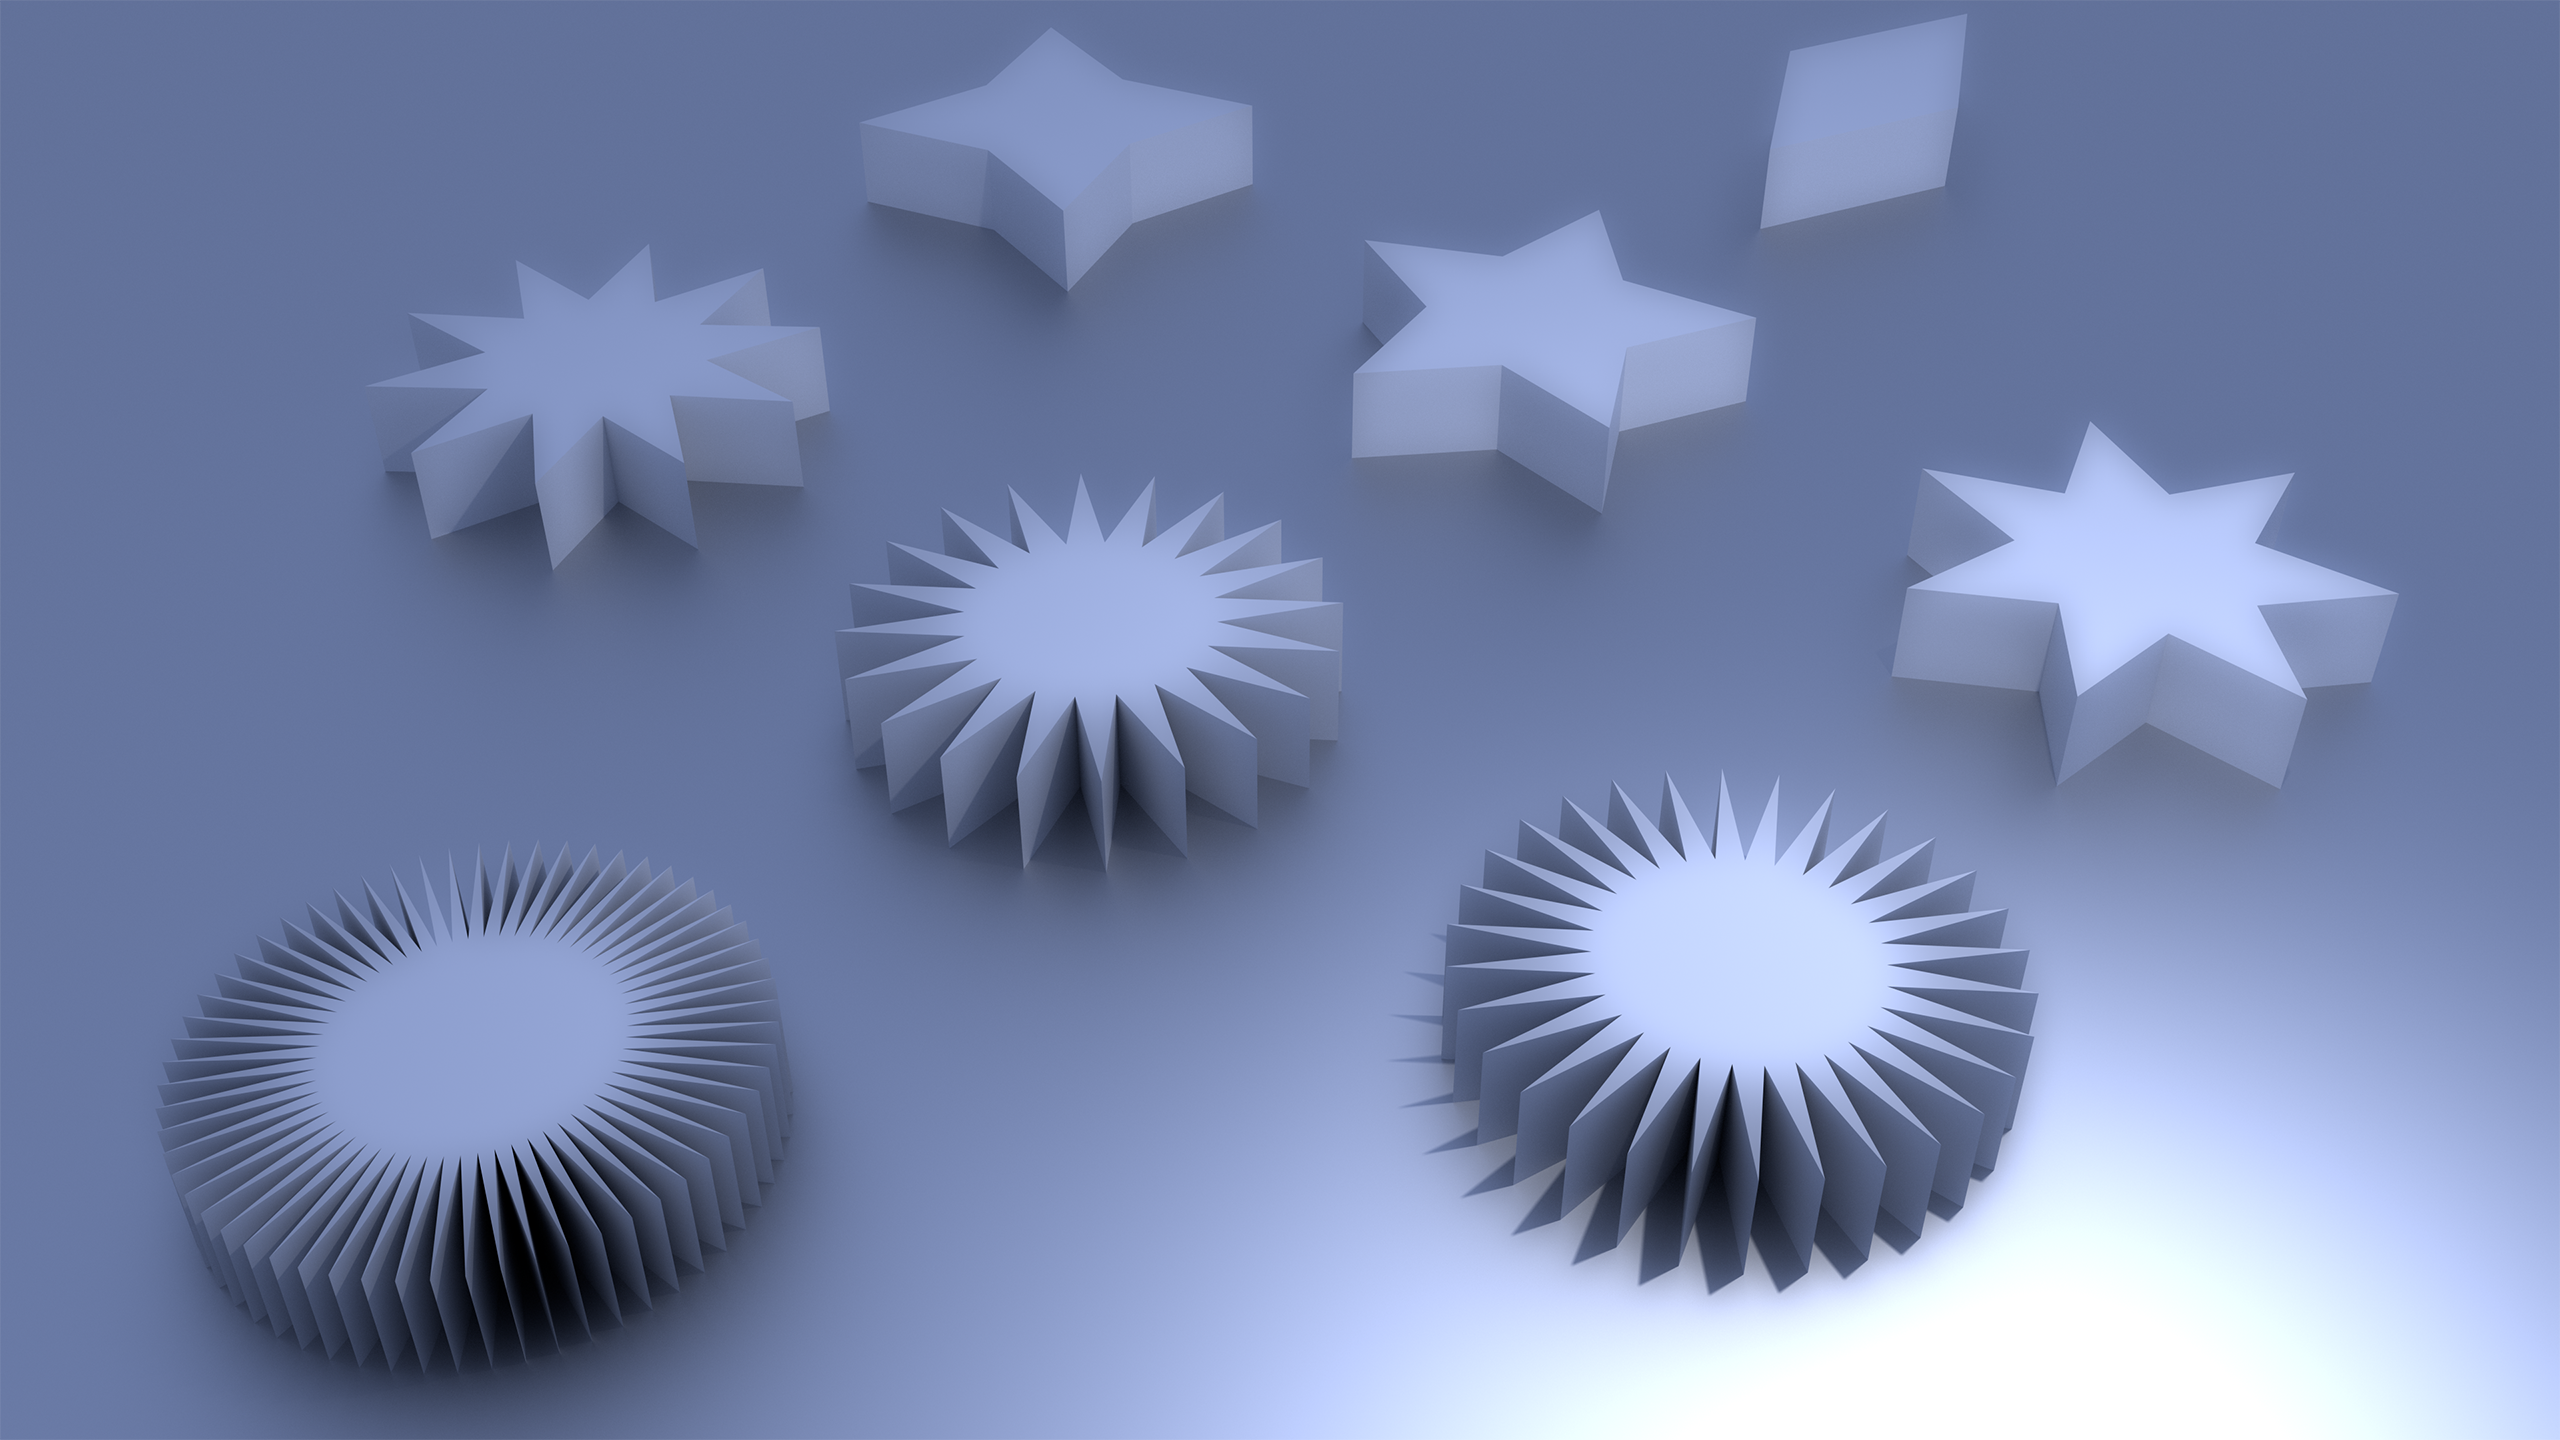
\includegraphics[width=.44\textwidth]{entwurf/star_2-4-5-7-10-20-30-60}}
			{\caption{Gute Unterscheidung von vorn}\label{fig:formen:sterne3d:front}}%
		\end{subfloatrow}
		\hspace*{\columnsep}%
		\begin{subfloatrow}
			\hsize0.7\hsize
			\vbox {%
				\ffigbox[\FBwidth][\FBheight]
				{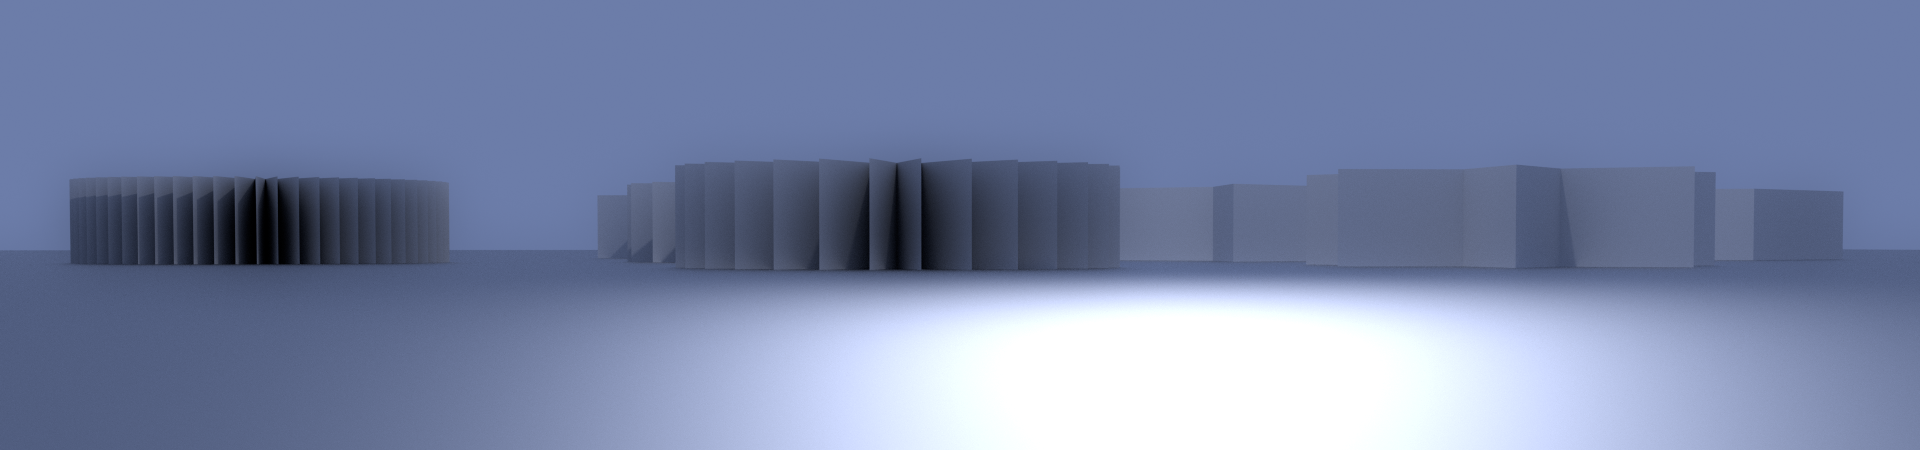
\includegraphics[width=.41\textwidth]{entwurf/star_2-4-5-7-10-20-30-60-seite}}
				{\caption{Die Unterschiede von der Seite \ldots}\label{fig:formen:sterne3d:side}}\vss
				\ffigbox[\FBwidth][\FBheight]
				{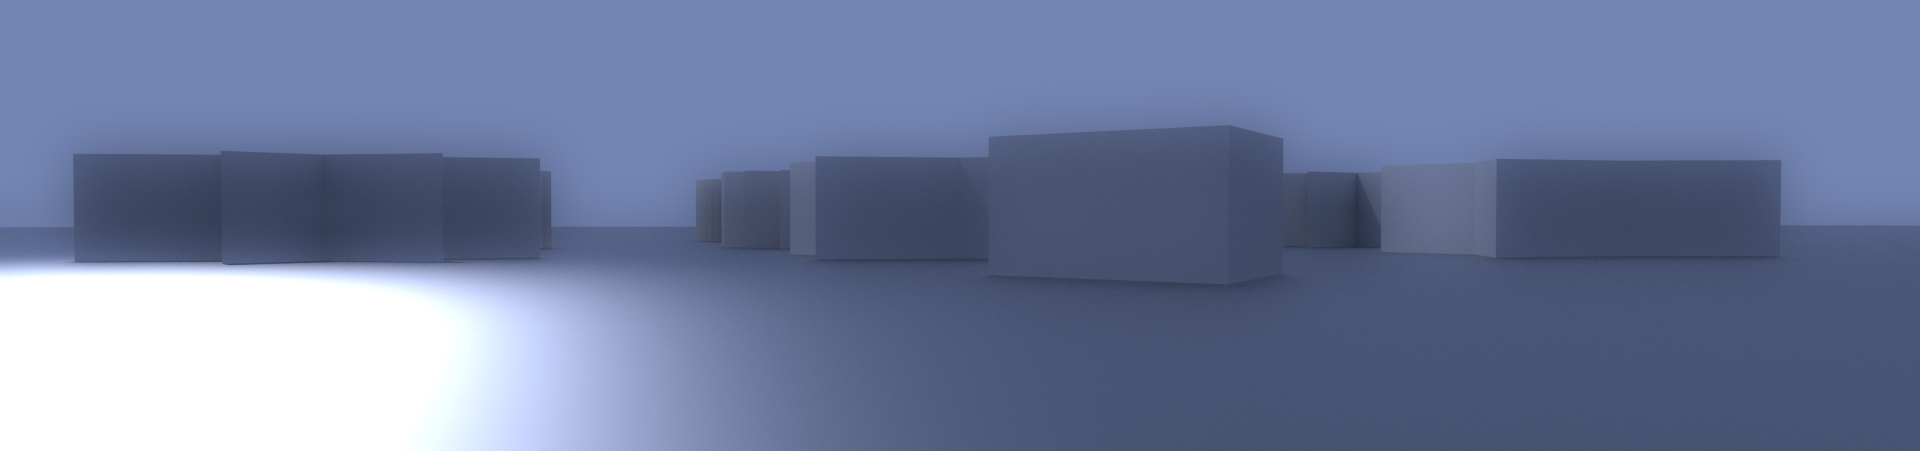
\includegraphics[width=.41\textwidth]{entwurf/star_2-4-5-7-10-20-30-60-oben}}
				{\caption{\ldots bzw. von oben sind kleiner.}\label{fig:formen:sterne3d:top}}
			}
		\end{subfloatrow}
	}
	{\caption{Formgebung mit sternenförmigem, nichtkonvexen Prisma. ERKENNBARKEIT SCHLECHTER ALS BEI TRANS UNTEN?}\label{fig:formen:sterne3d}}
\end{figure}

\begin{figure}
	\ffigbox[\FBwidth] {
		\begin{subfloatrow}
			\ffigbox[\FBwidth][]
			{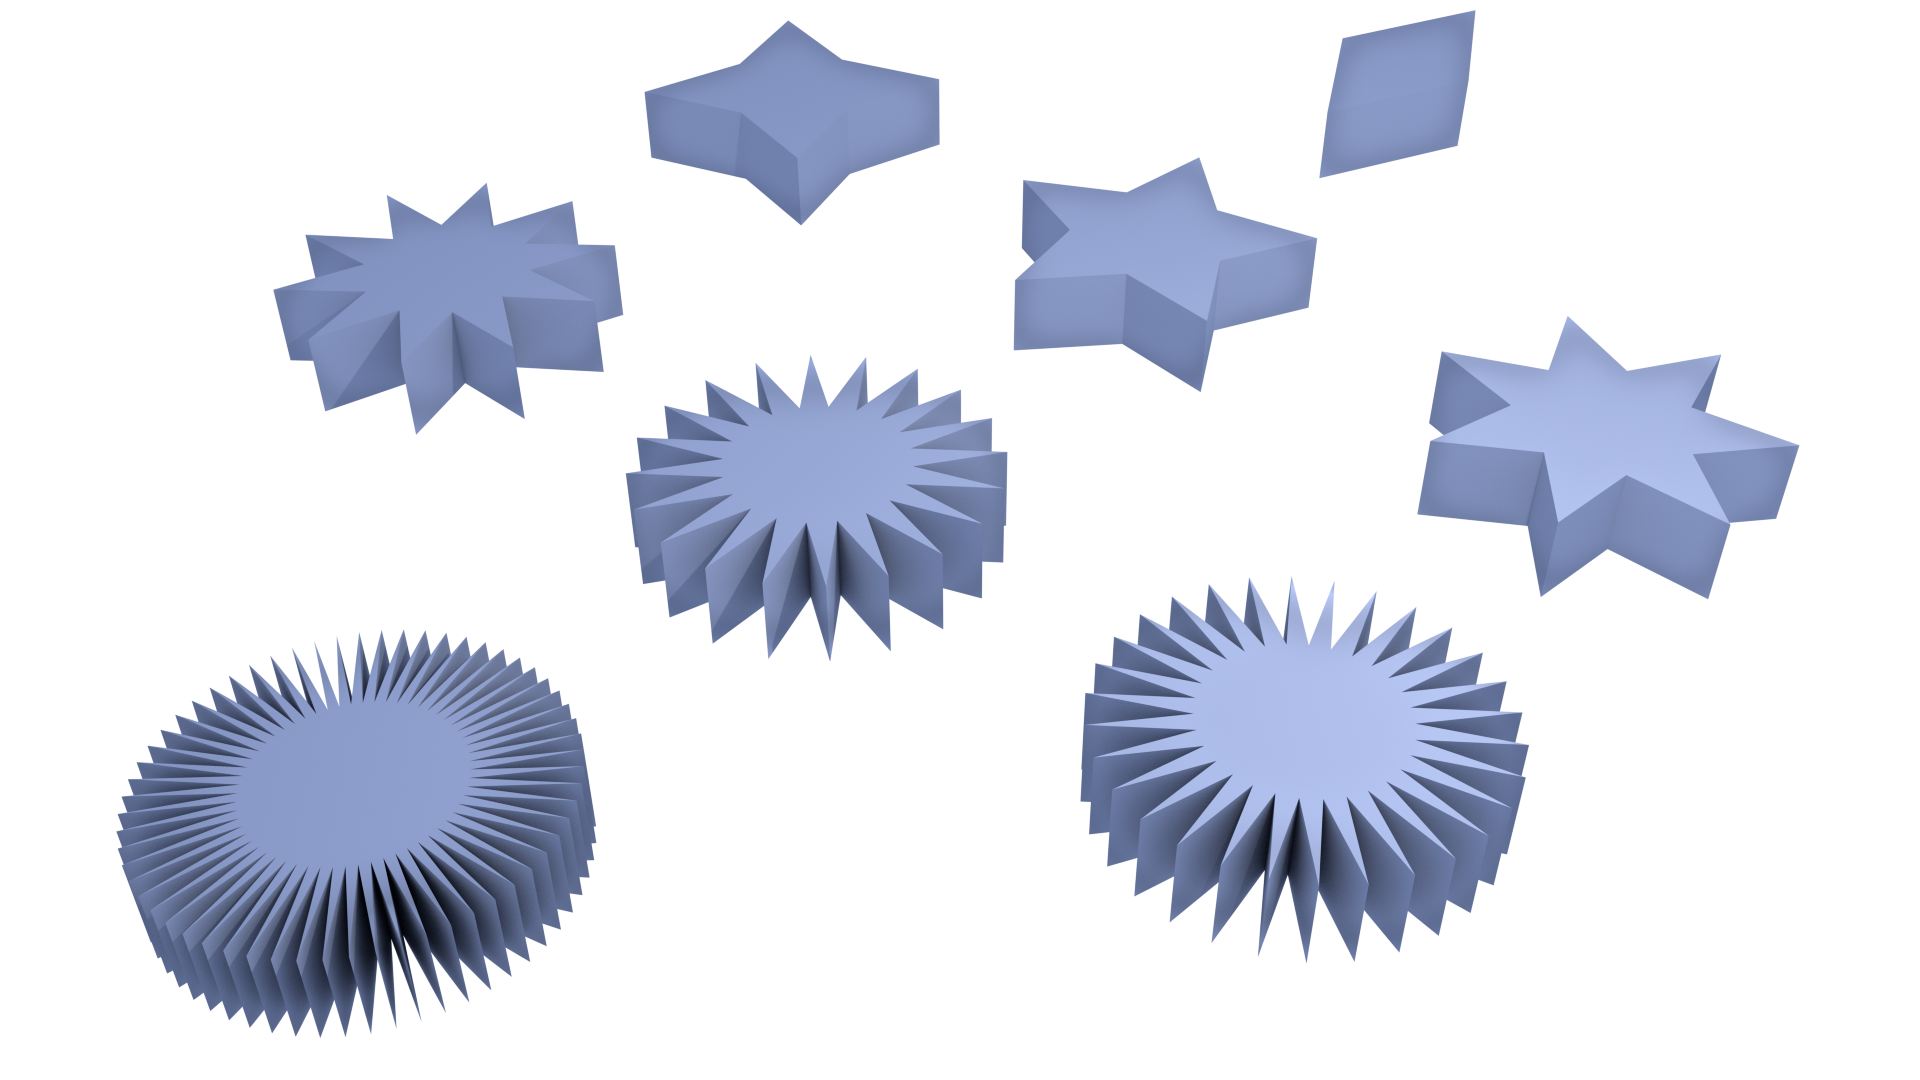
\includegraphics[width=.44\textwidth]{entwurf/star_2-4-5-7-10-20-30-60-trans}}
			{\caption{Gute Unterscheidung von vorn}\label{fig:formen:sterne3d:front-trans}}%
		\end{subfloatrow}
		\hspace*{\columnsep}%
		\begin{subfloatrow}
			\hsize0.7\hsize
			\vbox {%
				\ffigbox[\FBwidth][\FBheight]
				{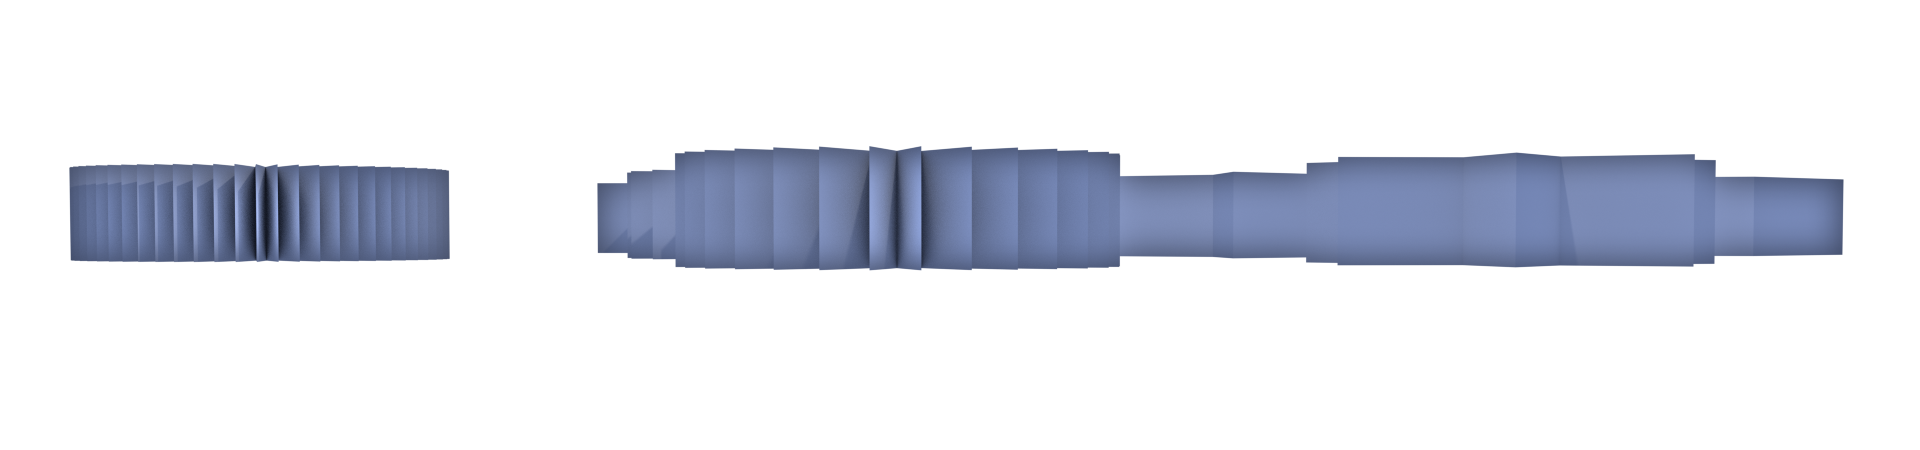
\includegraphics[width=.41\textwidth]{entwurf/star_2-4-5-7-10-20-30-60-seite-trans}}
				{\caption{Die Unterschiede von der Seite \ldots}\label{fig:formen:sterne3d:side-trans}}\vss
				\ffigbox[\FBwidth][\FBheight]
				{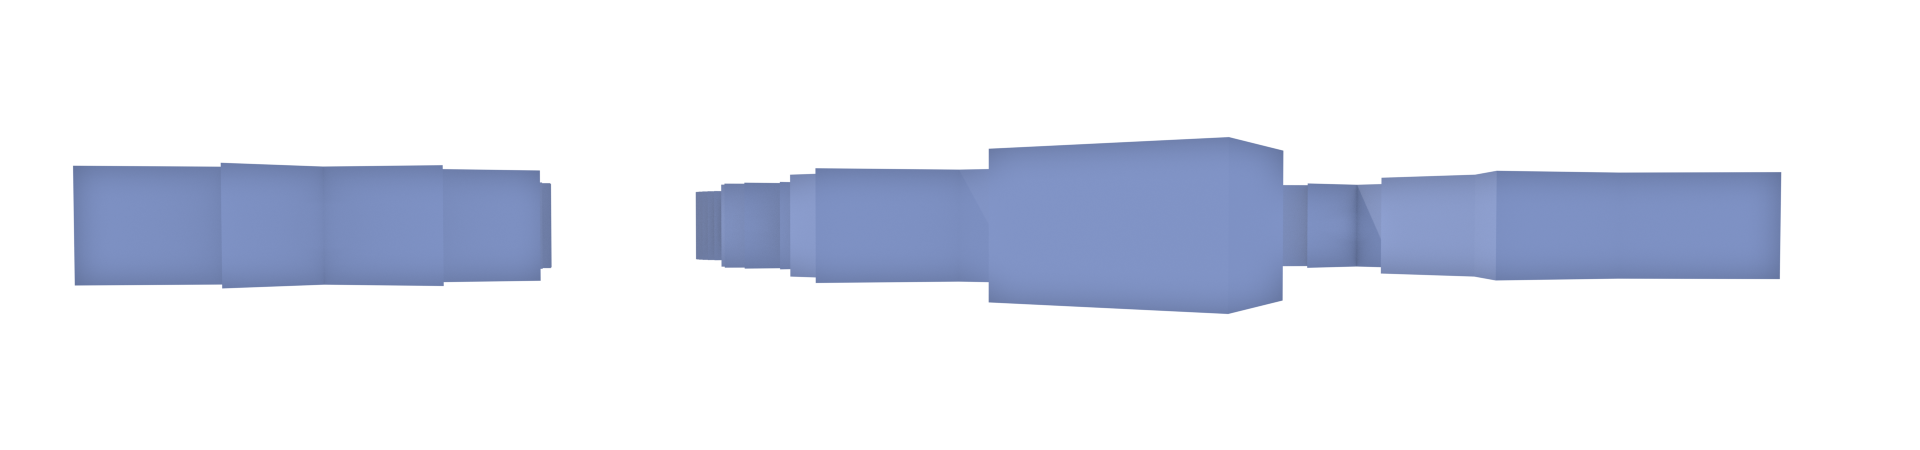
\includegraphics[width=.41\textwidth]{entwurf/star_2-4-5-7-10-20-30-60-oben-trans}}
				{\caption{\ldots bzw. von oben sind kleiner.}\label{fig:formen:sterne3d:top-trans}}
			}
		\end{subfloatrow}
	}
	{\caption{Formgebung mit sternenförmigem, nichtkonvexen Prisma. TRANSPARENT}\label{fig:formen:sterne3d-trans}}
\end{figure}

Die Anforderung, eine Formgebung zu wählen, die einen ähnlichen Umkugelradius und damit eine einheitliche Größe erhält, einen aus allen Winkeln ähnlichen Durchmesser sowie eine ähnliche Form aufweist, führt zu bestimmten Gruppen von Polyedern. Polyeder sind dreidimensionale Polytope und im engeren Sinne eine Teilmenge des \gls{3dRaum}, welche ausschließlich durch gerade Flächen begrenzt wird. Darunter zählen unter anderem die fünf \propernames{platonischen}{platonischer Körper} \cite{RegularPolyhedra}, die 13 \propernames{archimedischen}{archimedischer Körper}, die 13 \propernames{catalanischen}{catalanischer Körper} sowie die 92 \propername{Johnson-Körper} \cite{JohnsonPolyeder}. Eine Charakteristik dieser Polyeder ist ihre konvexe Form, was gleichzeitig die Unterscheidung aus der Distanz erschwert. Die prismatischen Polyeder fallen ebenfalls unter diese Kategorie, werden jedoch aus denselben Gründen ausgeschlossen wie die sternenförmigen Prismen.

Andererseits erfüllen die sternförmigen \propername{Kepler-Poinsot-Körper} (,,Sternpolyeder'') die Anforderungen. Sie besitzen im Gegensatz zu den vorgenannten Polyedern auch konkave Flächen \cite{KeplerPoinsotSolid} und können daher, wie in der interaktiven Visualisierung von \cite{WebGLUniformPolyhedra} zu sehen, leicht von den konvexen Polyedern unterschieden werden.

Ebenfalls geeignet ist der Vorschlag, eine Sternform durch sogenanntes \textquote{Poken} zu erzeugen: \blockcquote[4]{ProceduralGenerationofSculpturalForms}{By “poke” we mean a function to create a pyramid on each face of a given object. (This is different from Kepler’s stellation operation, which extends the face planes.)}

Somit gibt es mit der auf nichtprismatischen Polyedern basierenden Formgebung eine hohe Anzahl verschiedener Formen, die alle die Anforderung an eine einheitliche Größe, an einen aus allen Blickwinkeln ähnlichen Durchmesser und an die Wiedererkennbarkeit gewährleisten. Lediglich die Unterscheidung innerhalb der konvexen Polyeder kann schwerfallen. Am Deutlichsten unterscheiden sich die \propernames{platonischen Körper}{platonischer Körper} untereinander sowie die konvexen von den konkaven, sternförmigen Polyedern.


\subsubsection{Zweidimensionale Formgebung}\label{sec:related-2dformgebung}

siehe Quellen oder auch Grundlagen aus Kaptiel zwei



\chapter{Überblick}

Diese Arbeit stellt eine auf den Ideen der Skelettextraktion und Konturbäumen aufbauende Möglichkeit vor, um aus Punktdaten Strukturen zu erkennen. Diese Strukturen werden genutzt, um daraus Strukturereignisse abzuleiten.

Weiterhin werden %TODO, verwandte Arbeiten Visualisierung heranziehen

%TODO Nach Fertigstellung der Einleitung anpassen: %Die Arbeit behandelt zwei voneinander unabhängige Bereiche. Zum Einen werden Elemente eines Vektorraumes in Gruppen zusammengefasst und anhand dieser Gruppen heuristische Bestimmungen durchgeführt, zum Anderen werden diese Ergebnisse innerhalb des Vektorraumes dargestellt. Der erste Abschnitt dieses Kapitels beinhaltet Arbeiten zur Erkennung von Strukturen, der Zweite die Erstellung grafischer Elemente.

Die Schwerpunkte werden der Reihenfolge nach behandelt, wobei die Erkennung der Cluster- und Strukturereignisse zusammengefasst werden. Anschließend wird die Visualisierung der Ereignisse betrachtet.

Erklärung der Abschnitte, Module, Visualisierung.

Dateigröße von Datensätzen, Echtzeitdarstellung

\section{Beschreibung der Simulation}

Die dieser Arbeit zugrundeliegende Animation simuliert eine von einem Vakuum umgebenen Flüssigkeit, die rasch expandiert. Bedingt durch das quaderförmige, längliche Simulationsvolumen und der vollständigen Füllung mit Flüssigkeit in die zwei kurzen Raumrichtungen des Quaders sowie deren zentrale Positionierung, entstehen zwei Flüssigkeitsfronten, die entlang der langen Raumrichtung des Simulationsgebiets entgegengesetzt auseinander driften. Dazwischen entstehen Filamente und Tröpfchen und Gas durch sich aus den Fronten lösende Partikel und Partikelagglomerationen. Der Begriff Filament beschreibt dabei, dass es sich um Gebilde handelt, die im Vergleich zu ihrer Länge dünn sind. Tröpfchen sind von den Fronten unabhängige Gebilde mit eher kugelartiger Form. In den Leerräumen dazwischen befindet sich Gas. Die Gasphase wird dadurch definiert, dass alle Partikel große Abstände zueinander haben und sich beispielsweise gegenseitig nicht berühren.

Mit zunehmender Entfernung der Flüssigkeitsfronten zerreißen die Filamente zunehmend. Bei Zeitschritt 89 kollidieren beide Fronten miteinander, vermischen sich und driften etwa ab Zeitschritt 94 wiederholt auseinander. Das geschieht, weil das Simulationsvolumen periodische Randbedingungen aufweist. Zur Vereinfachung der Vorstellung kann der Quader als Ring betrachtet werden, auch wenn dieses Bild die Periodizität der anderen beiden Raumrichtungen nicht berücksichtigt.

Nach die Kollision bewegen sich beide Fronten in die entgegensetzte Richtung ,,zurück''. Dabei fangen sie vor der Kollision gebildete Filamente und Tröpfchen und hinterlassen ,,hinter'' sich vor allem Tröpfchen. Die Animation endet mit Zeitschritt 149, bevor sich die Fronten noch einmal begegnen.


%\chapter{Grundlagen}
%auf Skelett/Contour nicht eingehen, nicht verwendet.

%\section{kD Bäume}
%TODO kd Baum

%\section{Heuristik}
%TODO evtl
%TODO evtl was aus verwandte Arbeiten des Glyphdesigns hier rein





\chapter{Erkennung der Cluster und Strukturereignisse}

Die Erkennung wird in vier Schritte unterteilt. Als erstes wird eine Partikelliste erstellt und in dieser werden Informationen über die benachbarten Partikel hinterlassen. Als nächstes werden unter Nutzung dieser Nachbarschaftsverhältnisse Cluster erstellt und anschließend diese Cluster über zwei aufeinanderfolgende Zeitschritte verglichen. Als vierter und letzter Schritt folgt die Erkennung der Strukturereignisse über eine Heuristik, die den Vergleich aus Schritt drei nutzt. Eine detaillierte Liste findet sich in \autoref{sec:cluster-ereignis-schritte}.

Zuvor werden die zugrundeliegenden Daten und die genutzten Datenstrukturen beschrieben.

\section{Datenbehandlung}\label{sec:datenbehandlung}

%Das zum Konturbaum vergleichbare Skalarfeld wird aus den Abstandswerten der Partikel zum Rand desjenigen Clusters gebildet, in dem sie sich befinden. Daher wird die Bezeichnung \contour{Tiefenwert} für die Werte des Skalarfeldes verwendet. Sämtliche Partikel des Datensatzes sind Teil des Skalarfeldes, auch diejenigen der Gasphase außerhalb von Clustern.

Es liegen diskrete Eingangsdaten mit Partikeln mit definierten und disjunkten Positionen vor. Bis auf die räumliche Nähe weisen sie keine Zusammenhänge auf. Weiterhin existiert ein Funktionswert für jeden Partikel in Form einer vorzeichenbehafteten Entfernungsangabe. Dieser wurde mit Hilfe der Grenzen zwischen der flüssigen Phase und dem Vakuum bzw. der Gasphase bestimmt. Anschließend wird auf dieser Basis eine vorzeichenbehaftete Distanzfunktion aufgestellt, die für alle Partikel die Entfernung zum Rand bestimmt. Somit gibt der Funktionswert die Distanz zum nächsten Partikel an, welcher auf dem Rand eines Clusters liegt. Im Folgenden wird diese Größe als \contour{Tiefenwert} eines Partikels bezeichnet.

Partikel innerhalb von Clustern besitzen einen positiven \contour{Tiefenwert}, Partikel auf dem Rand weisen den Abstand null auf, Partikel in der Gasphase, d.h. außerhalb von Clustern, haben eine negative \contours{Tiefe}{Tiefenwert}.

Die Partikel-, Cluster- und Ereignisdaten werden als eine dichtgepackte Struktur gespeichert. So werden nur Datentypen mit vier und acht Byte verwendet, so dass der Compiler die Struktur wegen Ausrichtungsbeschränkungen im Speicher nicht auffüllt, wie es etwa bei ein Byte großen Datentypen passieren kann \cite{raymond1994cAlignment}. %TODO Tikz über Aufbau des Partikel- und des Cluster structs

Die Referenzen der Partikel untereinander sowie die der Partikel zu Clustern und umgekehrt werden mit Hilfe von Identifikatoren umgesetzt, die direkt in den Strukturen gespeichert sind. Dies hat Vorteile im Vergleich zur Nutzung von Zeigern als Referenz oder zur Speicherung der Objekte selbst. Letzteres erzeugt durch das Anlegen von Objektkopien Redundanz und kann daher zu inkonsistenten Daten führen. Weiterhin bedingt dies skalierend mit der Objektanzahl eine enorme Speicherbelastung und sorgte bei Tests auf dem Entwicklungssystem (siehe \autoref{sec:hardware}) zu ständigem Auslagern auf die Festplatte. Vorteile der Objektkopien sind der schnelle Zugriff auf die Daten sowie die Unabhängigkeit von Referenzen auf andere Objekte.
Die Verwendung von Zeigern ermöglicht einen unwesentlich langsameren Zugriff und es kann auf Kopien der referenzierten Objekte verzichtet werden. Allerdings darf sich bei Nutzung dieser Methode die Position der Objekte im Speicher nicht verändern, was je nach verfügbaren Ressourcen nicht garantiert werden kann und zu undefiniertem Verhalten führt. Denn es kann nicht ausgeschlossen werden, dass die Clusterliste im Speicher verschoben wird aufgrund der während der Laufzeit dynamisch allokierten und nicht vorhersagbaren Größe. So zeigen Tests %TODO Daten von createClusters_ptrAddress.log
, dass sich während der Clustererstellung die Position der Cluster im Speicher verändert, was dadurch bedingt ist, dass die gesamte Liste verschoben wird. Dies lässt sich an den ausgelesen Werten erkennen. So weist der Wert -572662307 beim Auslesen eines Integers darauf hin, dass der Speicherallokator einer Liste diesen Wert gesetzt haben könnte und was wiederrum sagt, dass sich vorher eine Liste in diesem Speicherbereich befunden haben könnte.

Um dem Problem zu begegnen, werden statt Zeigern Identifikatoren eingesetzt. %TODO Siehe ID im Schema Partikel/Clusteraufbau
Diese Identifikatoren werden genutzt, um zur Referenzierung auf die Listenzeiger zurückgreifen zu können. Die Methode hat drei Vorteile. Erstens ist die Geschwindigkeit nicht langsamer als mit einer direkten Zeigerreferenz, zweitens verweisen die Referenzen auch bei einer Verschiebung der die Objekte enthaltenen Listen im Speicher noch auf die korrekten Objekte und drittens kann geprüft werden, ob die Referenz mit dem im Speicher befindlichen Objekt übereinstimmt. Diese Prüfmöglichkeit ist dann wichtig, wenn die Objektlisten umsortiert werden. Zum Beispiel durch das Hinzufügen oder Entfernen von Elementen, die sich nicht am Ende der Liste befinden.


\section{Schritt 1: Bestimmung der nächsten Nachbarn}\label{sec:nachbarschaftssuche}

Ausgehend von der in \autoref{sec:related:connectedContour} referenzierten Bestimmung von Zusammenhangskomponenten über einen Maximalabstand zwischen Punkten im Netz, der ohne Baumstrukturen auskommt, könnte hier ebenfalls eine radialbasierte Nachbarschaftsbeziehung verwendet werden. Diese wurde geprüft und aufgrund des hohen Zeitaufwandes, verursacht durch die Entfernungsbestimmung zwischen Partikeln, verworfen (siehe \autoref{sec:cluster-radial}).

Eine Einteilung des Raumes in ein Gitter abhängig des Partikelradius wäre eine weitere Option. Einen ähnlichen Ansatz nutzt der kD-Baum, der die Partikel abhängig von ihrer Position in seine Äste verteilt und dadurch die Suche nach benachbarten Partikeln stark beschleunigt. Die Nutzung des Baumes bietet sich an, da die Anzahl der Partikel und ihre Positionen sich während eines Zeitschrittes nicht verändern und der Baum somit nicht modifiziert werden muss. Der Baum hat aufgrund der drei Raumrichtungen die Dimension $k=3$. Die Identifikation der Partikel erfolgt über den im kD-Baum eingetragenen Index, der der Position der Partikel in der Partikelliste entspricht. Daher wird während der Laufzeit über den beim Partikel gespeicherten Identifikator überprüft, ob die Reihenfolge der Liste modifiziert wurde, um Falschzuweisungen registrieren zu können.

Die periodischen Randbedingungen des Datensatzes werden standardmäßig beachtet, indem die Nachbarschaftssuche für jeden Partikel achtmal durchgeführt wird. Dabei wird die Position des Partikels für jede Raumrichtung auf die gegenüberliegende Seite des Simulationsvolumens versetzt, was bei drei Raumrichtungen acht Kombinationen ergibt.
Für Datensätze ohne periodische Randbedingungen kann der Nutzer dieses Vorgehen deaktivieren, so dass nur die Originalposition des Partikels verwendet wird.

Von der \tool{ANN}-Bibliothek wird die radienbasierte Suche annkFRsearch verwendet, da sich so eine Reichweite bestimmen lässt (vgl. \autoref{sec:related:connectedContour}). Als Suchparameter werden neben dem Radius selbst auch eine maximale Anzahl von zu prüfenden Nachbarn festgelegt. Dies ist nötig, da die \tool{ANN}-Bibliothek die Größe des Containers zur Speicherung der Identifikatoren der festgestellten Nachbarn (Nachbarschaftsliste) im Voraus festlegt. Dieser Wert wird abhängig vom Radius durch die Berechnung automatisch gesetzt. Die passenden Werte wurden experimentell bestimmt und erfüllen die beiden Voraussetzungen, dass alle im durch den Radius definierten Volumen befindlichen Artikel in die Nachbarschaftsliste aufgenommen werden können und andererseits möglichst wenig zusätzlicher, unnötiger Speicherplatz für den bei der Suche verwendeten Container für das Aufnehmen der Nachbarn reserviert wird. Die in \autoref{???} aufgeführten Werte wurden durch ein empirisches Annäherungsverfahren ermittelt. %TODO Ergebnisse des Experiments anhängen bzw. untenstehende Liste als Tabelle reicht.

	/// Minimal maxNeighbours for radius so no particle in radius gets excluded (determined by experiments):
	/// radiusModifier, maxNeighbours
	/// 4, 35
	/// 5, 60
	/// 6, 100
	/// 7, 155
	/// 10, 425
	/// 20, 3270

Der Suchradius wird durch den Nutzer einstellbar gestaltet, da mit der Reichweite der Nachbarschaftssuche die Anzahl der Cluster beeinflusst wird (siehe \autoref{sec:eva:nachbarschaftssuche}).

Die Suche wird für jeden Partikel durchgeführt. Dabei werden die Identifikatoren der gefundenen Nachbarn in die dafür vorgesehene Liste jedes Partikelobjekts hinzugefügt (siehe \autoref{sec:datenbehandlung}). Zuvor werden alle Partikel des \gls{mmpld} aus dem eingehenden \gls{mpdc} in diese Partikelobjekte umgewandelt und in die Partikelliste geshrieben. Da bekannt ist, wieviele Elemente der \gls{mmpld} enthält, findet eine Speicherplatzreservierung der Partikelliste statt, um eine Reallokation während der Eintragung der Partikel zu vermeiden.

Mit der Erzeugung dieser Partikelliste, der Eintragung aller Partikel in den kD-Baum und der Eintragung der Nachbarn in die Partikelobjekte ist der erste Schritt für die Berechnung der Strukturereignisse abgeschlossen und es folgt die Clusterbestimmung.

\section{Schritt 2a: Cluster-Fast-Depth Algorithmus zur Bestimmung der Cluster}\label{sec:fast-depth}

Zur Clusterbestimmung wurde der \gls{cfd}\index{CFD-Algorithmus} entwickelt. Der Begriff wurde ausgehend von der Nutzung des \contours{Tiefenwertes}{Tiefenwert} gewählt, angelehnt an die Depth-First Suche in Baumstrukturen.

Da auch Verschmelzungen und Teilungen innerhalb von Zusammenhangskomponenten erkannt werden sollen, genügt es nicht, wenn die Clusterbildung alle benachbarten Partikel einer Gruppe zuordnet. Vielmehr sollen auch Zusammenhangskomponenten selbst unterteilt werden.
%TODO Bilder mit den Zahlen innerhalb der Komponenten vom Vortrag einfügen
Dabei wird die Idee des Reebgraphen sowie die Bildung des Verbindungsbaumes beim Abtastalgorithmus der Konturbäume (siehe \autoref{sec:related:konturAbtast}) aufgegriffen und es werden kritische Punkte im Skalarfeld aller Partikel gesucht. Im Gegensatz zu den beiden genannten Ansätzen wird die Suche auf lokale Maxima beschränkt. Dies erfüllt die Anforderung, Partikel einer Zusammenhangskomponente in Gruppen zu unterteilen und ermöglicht zudem eine hohe Geschwindigkeit.

Die Partikelliste wird iterativ durchlaufen. Dabei werden die bei der Nachbarschaftssuche erstellten Beziehungen zwischen Partikeln genutzt, um für jeden Partikel denjenigen Nachbarn zu finden, der den höchsten \contour{Tiefenwert} aufweist. Ist dieser Nachbar gefunden, werden für diesen noch einmal alle Nachbarn nach dem ,,tiefsten'' durchsucht und dasselbe für diesen Partikel durchgeführt. Diese Suche geschieht ebenfalls iterativ. Sobald die umliegenden Partikel nur noch den gleichen oder einen geringeren \contour{Tiefenwert} als den des zuletzt betrachteten Partikels aufweisen, gilt die Suche als abgeschlossen. Anschließend wird ein neuer Cluster erstellt mit diesem Partikel als Wurzelpartikel. Sollte bereits ein Cluster mit diesem Partikel als Wurzel existieren, so wird kein neuer Cluster erstellt. Danach werden der ursprüngliche Partikel als auch alle Partikel, die während des iterativen Ablaufs der tiefsten Nachbarn getroffen wurden, zum Cluster hinzugefügt. Dies geschieht, indem der Clusteridentifikator des neu erstellten oder bereits vorhandenen Clusters in das Referenzfeld der Partikel für ihren zugehörigen Cluster (vgl. \autoref{sec:datenbehandlung}) eingetragen wird. %TODO Schema mit Illustrator erstellen analog zum Vortrag

Die Traversion erstellt einen kürzesten Pfad vom Ausgangspartikel zum Partikel mit der größten, lokalen Tiefe, wovon sich der Name für diesen Algorithmus ableitet. Da alle bei der Traversion getroffenen Partikel zum Cluster hinzugefügt werden und Partikel, kann der Algorithmus beschleunigt werden. Bevor die Fast-Depth Suche begonnen wird, wird der aktuell betrachtete Partikel auf seine Clusterzugehörigkeit geprüft. Sollte er einem Cluster angehören, so wird die Suche nicht erst begonnen, sondern es wird zum nächsten Partikel gesprungen.

Weiterhin werden Gaspartikel anhand ihres \contours{Tiefenwertes}{Tiefenwert} erkannt und übersprungen. Auch Partikel ohne Nachbarn werden übersprungen. Diese Überprüfung scheint redundant, jedoch können bei sehr kleinen Suchradien der Nachbarschaftssuche auch Flüssigkeitspartikel keine Nachbarn aufweisen, deren fehlende Nachbarschaft dann die Bedingung für Cluster, einer Zusammenhangskomponente anzugehören, nicht erfüllen würde.

Damit ist der wesentliche Teil der Clusterbildung abgeschlossen. Der zweite Schritt beinhaltet lediglich noch eine Reduktion kleiner Cluster. Die Definition für kleine Cluster kann dabei vom Nutzer getroffen werden.

%Obsolet
%Keine Sortierung wie beim vorgestellten Konturbaum. Sie ist teuer und würde den \CFDterm{Fast-Depth-Algorithmus} nicht beschleunigen. Stattdessen werden auf dem Pfad getroffene Partikel zum Cluster mit hinzugefügt.


\section{Schritt 2b: Reduzierung der kleinen Cluster}\label{sec:clusterreduktion}

Sehr kleine Cluster in den Zusammenhangskomponenten können unerwünschtes Rauschen in der Ereigniserkennung verursachen, so dass deren Partikel benachbarten, größeren Clustern zugewiesen werden. Ausgenommen sind diejenigen Cluster, die alleinig eine Zusammenhangskomponente bilden, auch wenn sie die Mindestgröße unterschreiten.

Es könnte eine Menge aus diesen sehr kleinen Clustern gebildet werden. Mit jedem Cluster diese Menge werden die naheliegensten ,,großen'' Cluster gesucht, zum Beispiel durch Anordnung der Rootpartikel der Cluster in einem kD-Baum. Allerdings ist eine Prüfung, ob sich die Cluster in einer Zusammenhangskomponente befinden, sehr aufwändig.

Aufgrund dessen, dass sich in der Arbeit auf eine kleine Mindestclustergrößen von zehn Partikeln beschränkt wird, kann eine iterative Prüfung auf benachbarte, große Cluster unter Nutzung der bestehenden Nachbarschaftsbeziehungen der Partikel genutzt werden. Dabei werden bei jedem Partikel, der ein Flüssigkeitspartikel mit Nachbarn ist und dessen referenzierter Cluster die Mindestclustergröße unterschreitet, die Nachbarn durchsucht. Sollten die Nachbarn alle keinem, demselben oder einem anderen sehr kleinen Cluster angehören, wird mit ihren Nachbarpartikeln die selbe Suche durchgeführt. In der aktuellen Implementation wird diese Suche maximal dreimal durchgeführt, so dass ausgehend vom ursprünglich betrachteten Partikel der maximal drittentfernteste Nachbar nach anderen Cluster durchsucht wird. Sollten zuvor schon andere Cluster gefunden worden sein, wird die Suche bereits dort abgebrochen. Nachbarpartikel, die keinem Cluster angehören (hier vor allem Gaspartikel, siehe \autoref{sec:fast-depth}), werden übersprungen.

Sollte nach Abschluss dieser Suche kein anderer, ,,großer'' Cluster gefunden sein, wird der sehr kleine Cluster bestehen gelassen, da dann davon ausgegangen wird, dass der Cluster eine Zusammenhangskomponente bildet und daher mit keinem anderen Cluster verschmolzen werden kann. Diese Annahme ist für eine Mindestclustergröße von zehn berechtigt, denn bei der dichten Struktur der Partikel in der Flüssigkeit erreicht spätestens die zweite Nachbarschaftsebene diese Anzahl an Partikeln. Der dritte Suchlauf dient als Puffer für etwas größere Mindestclustergrößeneinstellungen.

Sollte ein Cluster gefunden worden sein, so wird der betrachtete Partikel diesem Cluster zugeordnet. Die getroffenen Nachbarn werden nicht hinzugefügt, um die Schleife in mehreren Prozessen ohne Mutex ablaufen lassen zu können. Sollten mehrere Cluster gefunden worden sein, wird eine Entscheidung anhand der Richtung des Partikels zu den benachbarten Clustern bestimmt. Er wird zu demjenigen Cluster hinzugefügt, der am nächsten zur Richtung des Partikels zum Wurzelpartikel seines Clusters liegt.

Dazu wird der Winkel zwischen der Richtung vom Wurzelpartikel des betrachteten Partikel und seiner Position zur Richtung des Partikels zum in Frage kommenden Cluster berechnet. Dies wird für alle benachbarten Cluster durchgeführt. Der benachbarte Cluster mit dem geringsten Winkel im Intervall $[0, \pi]$ wird der neue Cluster des Partikels.

Da die Partikel voneinander unabhängig sind, können sie parallel durchlaufen werden (Umsetzung mittels \tool{OpenMP}). Weiterhin wird die Winkelberechnung zu jedem benachbarten Cluster parallelisiert.
Die Cluster werden nicht aus der Clusterliste gelöscht, um die Referenzen auf die Liste nicht neu erstellen zu müssen. Stattdessen wird durch den Algorithmus ihre Partikelanzahl auf 0 reduziert (sollten alle Partikel neuen Clustern zugeordnet werden), so dass sie in den folgenden Schritten herausgefiltert werden können.

\section{Schritt 3: Bestimmung der Clusterzusammenhänge}\label{sec:clusterzusammenhaenge}
Zur Bestimmung der Ereignisse ist es notwendig, die Entwicklung der Cluster zu verfolgen. Dazu werden Cluster über zwei Zeitschritte hinweg miteinander verglichen. Dieser Berechnungsschritt wird als \SECC bezeichnet.

\subsection*{Clusternachbarschaftsgraph}
Eine Variante ist die Erzeugung eines Graphen, der den Zusammenhang zwischen den Clustern zeigt und die bestehenden Nachbarschaftsbeziehungen der Partikel nutzt. Dazu kann die Clusterzugehörigkeit der Nachbarn jedes Partikel untersucht werden. Sollte ein Nachbar einem anderen Cluster angehören als der aktuelle Partikel, so sind der Cluster des aktuellen und der Cluster des benachbarten Partikels zusammengehörig. Durch Begrenzung auf Partikel mit geringen \contours{Tiefenwerten}{Tiefenwert} kann diese Suche stark beschleunigt werden und dennoch alle Nachbarschaftsbeziehungen gefunden werden, da einerseits der \CFD vor allem in die Tiefe und wenig in die Breite sucht und andererseits diese Beziehungen zwischen zwei Clustern aus beiden Richtungen geprüft werden.
Weiter soll darauf nicht eingegangen werden, da die Schwierigkeit dieser Variante in der Clusteridentifizierung über Zeitschritte hinweg besteht. Der Rootpartikel ändert sich von Zeitpunkt zu Zeitpunkt, die Partikelzugehörigkeit der Cluster ebenfalls (siehe \autoref{sec:eva:ereignisse}). Sie könnte als Ergänzung des hier implementierten Clustervergleichs dienen (siehe \autoref{sec:disc:optimierungAlg}.

\subsection*{Vergleich der zugehörigen Partikelmengen}
Ein direkteres Vorgehen, das unabhängig der Nachbarschaftsbeziehungen von Clustern ist, bietet der Vergleich der Partikelmengen der Cluster. Diese Methode greift die Idee des Volumenvergleichs für \contours{Isooberflächen}{Isooberfläche} von Konturbäumen auf \autoref{sec:related:konturbaumTemporal}. Die Cluster nehmen dabei die Position der \contours{Konturen}{Kontur} ein und die Partikel die Position des Gitters, da sie über ihren Identifikator eindeutig zugeordnet werden können. Weil hier keine kontinuierliche Fläche existiert, wird nicht von eingeschlossenem Volumen, sondern von Mengen gesprochen.

Zu jedem Cluster ist eine disjunkte Menge an Partikeln zugeordnet. Um diese Mengen über zwei Zeitschritte hinweg miteinander zu vergleichen, wird eine Matrix aufgebaut, deren Zeilen die Cluster des neuen Zeitschrittes enthalten und deren Spalten die Cluster des alten Zeitschrittes. Ein Partikel wird in diese \SECterm{Clustervergleichsmatrix} eingetragen, indem die Clusterzugehörigkeit des aktuellen Zeitschrittes sowie die Clusterzugehörigkeit des vorherigen Zeitschrittes ermittelt wird.

Anschließend werden zwei Schritte durchgeführt, um die für die Auswertung und schließlich die für die Eventerkennung notwendigen Werte zu ermitteln. In jedem Schritt werden alle Cluster eines Zeitschrittes betrachtet und für jeden werden Cluster des anderen Zeitschrittes gesucht, die mit dem betrachteten Cluster gemeinsame Partikel aufweisen. Diese werden als \SECterm{Partnercluster} bezeichnet. Im ersten Schritt werden alle derzeitigen Cluster mit jedem des vorherigen Zeitschrittes verglichen (vorwärtsgerichteter Vergleich), im zweiten Schritt alle vorherigen mit jedem Cluster des aktuellen Zeitschrittes (rückwärtsgerichteter Vergleich). 

Zur Speicherung der Vergleichsergebnisse wird eine Partnerclusterstruktur eingeführt. Diese enthält eine Liste der \SECterm{Partnercluster} zusammen mit den jeweils gemeinsamen Partikeln sowie Methoden zur Berechnung von Gesamt- und Durchschnittswerten. Für beide Vergleichsrichtungen werden diese Strukturen in separate Listen geschrieben. Damit lassen sich die Anzahl der gemeinsamen Partikel für jeden vorhergehenden Cluster und jeden aktuellen bestimmen, woraus sich die weiteren für die Analyse notwendigen Werte ermitteln lassen.

\section{Schritt 4: Erkennung von Ereignissen}\label{sec:ereigniserkennung}

Es wird jeweils ein Cluster und seine \SECterm{Partnercluster} betrachtet. Dies geschieht sowohl für den vorwärtsgerichteten als auch den rückwärtsgerichteten Vergleich.

Zur Analyse der durch die Partnerclusterstruktur zurückgegeben Daten wird ein heuristisches Vorgehen genutzt. Tests haben gezeigt, dass die Partikel selten in Clustern mit derselben Clusternummer bleiben. Das lässt sich damit erklären, dass die Clusterzuweisung stark von der Position der Partikel und ihrer Nachbarschaftsverhältnisse abhängen und diese sich durch die sich bewegenden Partikel von Zeitschritt zu Zeitschritt stark ändern. Somit ist der intuitiv wirkende Vergleich über den Clusteridentifikator für die Beobachtung von Veränderungen nicht möglich und kann ausgeschlossen werden. %TODO-- Testdaten
Dagegen kann ein Vergleich der Anteile von Partikeln in den Clustern erkennen lassen, ob sich der Zusammenhang zwischen den Partikeln verändert hat. Die für die Betrachtung relevante Clustereigenschaft ist die Anzahl der Partikel eines Clusters und wird als \SECterm{Clustergröße} bezeichnet.

Die Größe eines Clusters hat für die Relevanz von Ereignissen keine Bedeutung, da sie durch die Vorgehensweise der \CFD stark von der Topologie der Strukturen abhängt. Ein durch einen kleinen Cluster an einer Engstelle eines Filaments ausgelöstes Ereignis kann für die Analyse bedeutender sein als ein Ereignis innerhalb der Flüssigkeitsfront, ausgelöst durch große Cluster. Um die Abhängigkeit der Ereigniserkennung von der \SECterm{Clustergröße} zu eliminieren, werden relative Werte verwendet. 

Neben der Größe eines Cluster werden durch den \SECC folgende Werte bereitgestellt

Intuitiv

Betrachtete Faktoren:
- Relevanz: clusterSize (nicht unbedingt aussagekräftig, daher Prozentwerte)

- selber Cluster: getAveragePartnerCommonPercentage groß, getLocalMaxTotalPercentage groß, getNumberOfPartners klein

- Rauschen: getAveragePartnerCommonPercentage klein, getSmallPartnerAmount groß, LocalMaxTotal klein oder  getBigPartnerAmount(25) = 0

- Split: getBigPartnerAmount(25) > 1 (forward), evtl zusätzlich Partners sehr klein und getAveragePartnerCommonPercentage mittel (backwards) bei großen Clustern size und getCommonPercentage hoch

- Merge: getBigPartnerAmount(25) > 1, 25 für = 2 zu niedrig: 40, 35, 30, testen (backwards), bei großen Clustern size und getCommonPercentage hoch

- Birth: getNumberOfPartners = 0 (backwards) oder getTotalCommonPercentage < 10.

- Death: getNumberOfPartners = 0 (forward) oder getTotalCommonPercentage < 10.

Die für die Spliterkennung verwendete Methode erfasst nicht die Abspaltung von Clustern, die ??\% kleiner sind als der Ausgangscluster. Bei Merge ist es synonym.

Werte relativ zum Anteil der gemeinsamen Partikel, um kleine und große Cluster gleichermaßen zu behandeln.

CODING TODO vielleicht:
Beachtet werden muss ein Rauschen, welches durch ständiges Hinzufügen und Lösen von Randpartikeln eines Clusters besteht. Da dieses Rauschen mit zunehmender Clustergröße durch die höhere Anzahl an Randpartikeln verstärkt wird, werden die Betrachtungen mit prozentualen Werten durchgeführt. Andererseits können so große Cluster verstärkt in das Rauschen eingeteilt werden, so dass auch große \SECterm{Partnercluster} mit Werten kleiner als der festgelegte Grenzwert für Split und Merge Ereignisse in Betracht gezogen werden. Dabei wird getCommonPercentage auf hohe Werte untersucht.



Erste Vorgehensweise:
1) Vergleich eines vorhergehenden Clusters mit allen Folgenden (Spalte), Referenzclustergröße: alter Cluster
a) 0 gemeinsame (keine Partikel in einem Cluster): Death
b) 0 im Selben, viele/alle in (einem oder mehreren) anderen: Merge
c) Sehr viele/alle im Selben, wenige in anderen: Nichts passiert oder Merge (damit nicht feststellbar).
d) Hälfte im Selben, Hälfte in einem anderen oder verteilt: Split
Birth so nicht feststellbar.

2) Vergleich des aktuellen Clusters mit allen Vorhergehenden (Zeile), Referenzclustergröße: neuer Cluster
a) 0 gemeinsame (keine Partikel in vorhergehenden Clustern): Birth
b) Schritt (c) von (a) noch machen.
Death so nicht feststellbar.


\section{Speicherung der Daten}
%TODO raus hier
Umwandlung von framebehafteten MMPLD in frameloses MMSE.

Das \gls{mmse} enthält die berechneten Ereignisse in einem Bytecode fest. Der Vorteil im Vergleich zu JSON/XML oder anderen textbasierten Speicherverfahren ist die höhere Performance beim Lesen und Schreiben sowie die kleinere Dateigröße. Die Ereignisdaten sind dabei sequentiell abgelegt

\begin{figure} %todo Bild mmse
	\begin{tikzpicture}[]
	Header: Anzahl Events, Maximale Zeit, evtl max x,y,z Pos
	Daten: Position, Zeit, Typ (Agglo?)
	\end{tikzpicture}
	\caption{Datentypen}\label{fig:mmse:format}
\end{figure}

\section{Programmaufbau für die Berechnung}
%TODO raus hier, evtl in Anhang
%TODO Bild writer mmprj Aufbau

Speicherung der Clustervisualisierung durch MMPDC.

Auslösung der Berechnung für die unterschiedlichen Frames erfolgt durch den verbundenen SimpleSphereRenderer, da der aus der Calculation ausgehende MPDC für den Wechsel der Frames verantwortlich ist.

Call zur intermodularen Kommunikation. Sämtliche Listenelemente, auf die mit Zeigern zugegriffen wird - wie Partikel, Cluster und Strukturereignisse - sind dichtgepackte Strukturen mit Datentypen der Länge vier oder acht Byte, damit der Compiler kein zusätzliches Padding einfügt und so die Strides und damit die Pointer ungültig macht.

%TODO im Programm EVTL noch Automatisierung einbauen (Framesteuerung durch Calc)


\chapter{Visualisierung}\label{sec:visualisierung}

Dieses Kapitel beschreibt die Erstellung eines Mockups, das zum Einen zur möglichen Zuordnung der Ereignisparametern zu visuellen Attribute dient. Zum Anderen dient es zur Prüfung von dreidimensionalen Glyphen. Weiterhin werden die Umsetzung der Glyphgestaltung als auch der Glyphvisualisierung mit einem Renderer beschrieben sowie die Visualisierung der Cluster im Partikelraum.
Zur Einordnung der Darstellung in die Taxonomie von Gleicher et al (siehe \autoref{sec:related-visAnordnung}) werden der Partikel- und der Ereignisraum als zwei separate Objekte betrachtet. Dazu werden die Begriffe \vis{Partikelobjekt} und \vis{Ereignisobjekt} eingeführt. Der erste Begriff steht für die Visualisierung der Partikel und beinhaltet den gesamten Verlauf von 150 Zeitschritten. Der zweite steht für die Visualisierung der Ereignisse für alle Zeitschritte.  %Evtl in Grundlagen: Links auf diesen Abschnitt dann updaten!


\section{Mockup}%TODO entschlacken!!

\subsection{Taxonomie der Visualisierung}\label{sec:vis-taxonomie}
%TODO durch Glyphskalierung Häufung unwichtig, das aber wohl erwähnen
Die Berechnung des Clusterverhaltens ergibt eine Datenbank, in der Ereignisse abgelegt sind. Ein Ereignis stellt einen Datensatz dieser Datenbank dar, die Parameter des Ereignisses sind die Datensatzfelder. Die Aufgabe der Visualisierung ist es, den Parametern eines Ereignisses visuelle Attribute zuzuweisen. Diese Zuweisung kann in einer weiteren Datenbank als Relation %im Sinne des \gls{rdbms}
zwischen Parameter und Attribut festgehalten werden.

Zum leichteren Verständnis erfolgt eine Einteilung der Parameter, der Attribute sowie der Zuweisungen in die beiden in \autoref{fig:entwurf:taxonomie:vartype} gezeigten Variablentypen. Der Typ \propername{Zahlenwert} steht dabei für die Nutzung eines kontinuierlichen Zahlenraumes, während der Variablentyp \propername{Vokabular} eine diskrete, beschränkte Zuordnung mit voneinander disjunkten Elementen beschreibt.

\begin{figure}
	\begin{tikzpicture}[]
	\node {Variablentyen im Entwurf}
	child { node [value] {Zahlenwert} }
	child { node [vocab] {Vokabular} };
	\end{tikzpicture}
	\caption{Taxonomie der Variablentypen}\label{fig:entwurf:taxonomie:vartype}
\end{figure}

\subsubsection{Parameter eines Ereignisses}
Ein Ereignis besteht aus drei Parametern, die jeweils zwischen ein bis drei Freiheitsgraden aufweisen.

\begin{itemize}
	\item Zeitpunkt: ein Wert (t)
	\item Ort: drei Werte (x, y, z)
	\item Art: ein Vokabular [Split, Merge, Death, Birth]
\end{itemize}

\subsubsection{Visuelle Attribute eines Ereigniselements}\label{sec:attribute}
Die visuellen Attribute können sowohl als fließender \propername{Zahlenwert} als auch als festes \propername{Vokabular} umgesetzt werden. Beispielsweise bedeutet der Vokabulartyp für das \visattrs{Positionsattribut}{Position} die Festlegung bestimmter Koordinaten für jeden Begriff des Vokabulars.

Jedes Attribut besitzt eine individuelle Anzahl an Freiheitsgraden, die zur Visualisierung genutzt werden können.

\begin{itemize}
	\item Position: 3 (x, y, z)
	\item Farbe: 2 (Farbwert/Sättigung, Helligkeit)
	\item Form: 1, eine Wertzuweisung ist möglich durch die Anzahl der Ecken, Kanten und Flächen. Anderes wie z.B. der Abstand der Ecken vom Körperzentrum kollidiert mit dem Attribut Größe.
	\item Größe: 1
	\item Opazität: 1
\end{itemize}

Da Farbwerte bei geringer Sättigung nicht mehr voneinander unterschieden werden können, werden diese beiden Farbeigenschaften zusammengefasst. Dadurch kann die Helligkeit leicht als separates Attribut vom Betrachter erkannt werden, wie in \autoref{fig:entwurf:farbtafel} zu sehen.

\begin{figure}
	VERGLEICHSBILD MIT WECHSELNDER SÄTTIGUNG UND HELLIGKEIT
	%\includegraphics[width=.8\textwidth]{entwurf/}
	\caption{Farbtafel mit unterschiedlicher Sättigung und Helligkeit}\label{fig:entwurf:farbtafel}
\end{figure}

Bei der \visattr{Form} sind mehrere Freiheitsgrade möglich, etwa eine Kombination aus Anzahl der Ecken mit einem variablen Abstand dieser vom Körperzentrum. Der variable Abstand kollidiert jedoch mit dem Attribut \visattr{Größe}. Daher wird das Attribut \visattr{Form} auf einen Freiheitsgrad beschränkt und es werden die in \autoref{sec:grundlagen:formgebung} beschriebenen Polyeder verwendet. Da die Anzahl an Polyedern begrenzt ist und die Unterscheidungsmöglichkeit mit zunehmender Flächenanzahl sinkt, ist das Attribut \visattr{Form} nur eingeschränkt als Zahlenwert verwendbar.

Bei der Bestimmung der Attribute wurde darauf geachtet, ein umfassendes Spektrum der Gestaltgesetze nutzen zu können. Alle visuellen Attribute fallen unter den Einfluss des \viss{Gesetzes der Prägnanz}{Gesetz der Prägnanz}. Mit der \visattr{Position} kann das \vis{Gesetz der Nähe} sowie das \vis{Gesetz der gemeinsamen Region} genutzt werden, eine Kombination aus der \visattr{Position} mit den anderen Attributen resultiert in der Verwendbarkeit des \viss{Gesetzes der Kontinuität}{Gesetz der Kontinuität}. Bis auf die \visattr{Position} kann mit allen visuellen Attributen das \vis{Gesetz der Ähnlichkeit} genutzt werden. Das \vis{Gesetz der Geschlossenheit} kann mit dem \visattrs{Positionsattributs}{Position} verarbeitet werden, falls durch entsprechende Zuweisung die Elemente nah beieinander lägen und sie eine geschlossene Form bilden. Mit den hier definierten Attributen kann somit von sechs der zehn in \autoref{sec:related-gestaltgesetze} aufgezählten Gestaltgesetze Gebrauch gemacht werden.

Texturen als ein eigenständiges visuelles Attribut werden ausgeklammert, da sie sich mit dem Attribut \visattr{Farbe} und bei der Nutzung als Oberflächenstruktur mit dem Attribut \visattr{Form} überschneiden. Ein Einsatz als Bump Map oder Displacement Map zur Unterstützung des Attributs \visattr{Form} wäre denkbar. Aufgrund dessen, dass bereit Polyeder für das \visattrs{Formattribut}{Form} genutzt werden, wird von einer Verwendung von Texturen allerdings abgesehen.

Animationen bieten weitere visuelle Attribute wie Bewegungsrichtung, Bewegungsbahn, Beschleunigung und Geschwindigkeit als auch die Veränderung der anderen Attribute und eröffnen damit die Nutzung des \viss{Gesetzes der Gleichzeitigkeit}{Gesetz der Gleichzeitigkeit} sowie des \viss{Gesetzes der gemeinsamen Bewegung}{Gesetz der gemeinsamen Bewegung}. Sie werden im Rahmen dieser Arbeit jedoch nicht behandelt.

Die visuellen Attribute lassen sich durch den Betrachter unterschiedlich gut unterscheiden. In der folgenden Sortierung nach ihrer Unterscheidungsgüte stehen die am Leichtesten zu unterscheidenden Attribute ganz oben. (QUELLE)
\begin{enumerate}
	\item Position
	\item Farbwert
	\item Größe
	\item Form
	\item Helligkeit
	\item Opazität
\end{enumerate}

Die Attribute mit höherer Unterscheidungsgüte sollten bevorzugt gewählt werden. Form, Helligkeit und Opazität sind durch die geringere Güte besser als Vokabular- denn als Wertattribut geeignet, da bei den Vokabularen die Anzahl der Begriffe im Vergleich zur Menge der Zahlenwerte gering ist. Dadurch können die Attributseigenschaften weiter auseinanderliegen, was eine leichtere Unterscheidung ermöglicht.

Die 

In der \tool{MegaMol} Molekularsimulation wird ausschließlich das visuelle Attribut \visattr{Position} zur Darstellung genutzt.

\begin{figure}
	\ffigbox[\FBwidth] {
		\begin{subfloatrow}
			\ffigbox[\FBwidth] {
				\fbox {
					\begin{tikzpicture}[level 1/.style={sibling distance=1.4cm}]
					\node {Ereignis}
					child { node [value] {Zeitpunkt} }
					child { node {Ort}
						child [verticalChild, first] { node [value] {x} }
						child [verticalChild, second] { node [value] {y} }
						child [verticalChild, third] { node [value] {z} }
					}
					child { node [vocab] {Art}
						child [verticalChild, first] { node {Split} }
						child [verticalChild, second] { node {Merge} }
						child [verticalChild, third] { node {Death} }
						child [verticalChild, fourth] { node {Birth} }
					};
					\end{tikzpicture}
				}
			}
			{\caption{Ereignis mit Variablentyp}\label{fig:entwurf:taxonomie:ereignis}}%
			
			\ffigbox[\FBwidth] {
				\fbox {
					\begin{tikzpicture}[level 1/.style={sibling distance=1.8cm}]
					\node {Visuelles Attribut}
					child { node {Position}
						child [verticalChild, first] { node [] {x} }
						child [verticalChild, second] { node [] {y} }
						child [verticalChild, third] { node [] {z} }
					}
					child { node {Farbe}
						child [verticalChild, first] { node [] {Farbwert \& S"attigung} }
						child [verticalChild, second] { node [] {Helligkeit} }
					}
					child { node [] {Größe} }
					child { node [] {Form}	}
					child { node [] {Opazität} }
					;
					\end{tikzpicture}
				}
			}
			{\caption{Die visuellen Attribute können beide Variablentypen annehmen.}\label{fig:entwurf:taxonomie:variable}}
		\end{subfloatrow}
	}
	{\caption{Taxonomie der Daten und visuellen Attribute}\label{fig:entwurf:taxonomie}}
\end{figure}

\subsubsection{Problem der lokalen und temporalen Agglomeration}\label{sec:entwurf:agglomeration}

Die Anzahl der Datensätze, die denselben Ort oder denselben Zeitpunkt aufweisen können, ist unbekannt. Schon eine geringe Anzahl identischer Orte oder Zeitpunkte kann je nach Zuordnung der visuellen Attribute zu einer überlagerten, nicht mehr unterscheidbaren Darstellung führen, wodurch die Erkennung solcher Agglomerate nicht gegeben ist. Daher wird ein visuelles Attribut reserviert, um eine solche Anhäufung von Ereignissen anzuzeigen. Die \dataparam{Häufung} wird bei der Zuweisung zu den visuellen Attributen wie ein Ereignisparameter behandelt. Abhängig von dieser Zuweisung in \autoref{sec:entwurf:zuweisung:parameter-attribut} können zwei Werte für die lokale und temporale Häufigkeit notwendig sein. Dieser wird jedem Ereignis zugewiesen und wird beim Auffinden von identischen Ortsparametern bzw. Zeitparametern in den Datensätzen inkrementiert.

Die Begriffe \dataparam{Agglomeration} und \dataparam{Häufung} sind hier synonym.

Bei der Visualisierung von Agglomeraten kann die natürliche Wirkung (QUELLE) der visuellen Attribute genutzt werden. Groß, opaque und dunkel stehen für eine starke Agglomeration. Klein, transparent und hell für eine niedrige.

\subsubsection{Verbundenheit}\label{sec:entwurf:verbundenheit}
Wenn sich ein Cluster teilt (Split) und sich die resultierenden Cluster wiederrum teilen oder mit anderen Clustern verschmelzen (Merge), so kann man diesen Ereignissen Vorgänger (Eltern) sowie Nachfolger (Kinder) zuordnen. IST DAS RICHTIG?

\vis{Gesetz der Geschlossenheit}
\vis{Gesetz der fortgesetzt durchgehenden Linie}
\vis{Gesetz der verbundenen Elemente}


\subsection{Parameter-Attributszuweisung}\label{sec:entwurf:zuweisung:parameter-attribut}

In der \propername{MegalMol} Simulation wird der Ort des Ereignisses mithilfe der Teilchenposition dynamisch visualisiert. Insofern kann angenommen werden, dass für eine nahtlose Benutzbarkeit zwischen der \tool{MegaMol} Animation und der statischen Visualisierung die Zuweisung des Elementattributes \visattr{Position} an den Parameter \dataparam{Ort} empfehlenswert ist. Weiterhin ist die Reservierung der \visattr{Opazität} für die \dataparam{Häufung} die einfachste Möglichkeit, denn dies hat zwei Vorteile. Zum Einen ist keine nachträgliche Modifizierung der visuellen Attribute der einzelnen Ereignisse notwendig, denn die Opazitätseigenschaft sorgt durch Überlagerung für eine von der Anzahl direkt abhängige Hintergrundverdeckung. Dadurch werden zum Anderen auch keine Informationen über die Häufigkeit im Datensatz benötigt. Hingegen muss zum Beispiel eine Größenveränderung nachträglich für jedes Ereignis im Agglomerat auf der Basis eines temporalen oder lokalen \dataparams{Häufungswert}{Häufung} durchgeführt werden.

Darüberhinaus wird jedem Ereignisparameter nur eine visuelles Attribut zugeordnet, denn Mehrfachzuweisungen sollten wegen einer Verminderung der präattentiven Wahrnehmung (VERWEIS AUF GRUNDLAGEN) vermieden werden.

Daraus ergeben sich die in \autoref{tab:entwurf:zuweisung-param-attr:position-agglo} aufgeführten Visualisierungsmöglichkeiten.

\begin{table} 
	\begin{tabularx}{\textwidth}{@{}CCCCCCCCC@{}}
		\toprule
		Attribute & Position x & Position y & Position z & Farbwert \& Sättigung & Helligkeit & Eckenanzahl & Größe & Opazität \tabularnewline
		\midrule
		& Ort x & Ort y & Ort z & Art & Zeit & & & H \tabularnewline
		& Ort x & Ort y & Ort z & Art & & Zeit & & H \tabularnewline 
		& Ort x & Ort y & Ort z & Art & & & Zeit & H \tabularnewline 
		& Ort x & Ort y & Ort z & Art & & & & H \tabularnewline 
		\midrule
		& Ort x & Ort y & Ort z & Zeit & Art & & & H \tabularnewline 
		& Ort x & Ort y & Ort z & & Art & Zeit & & H \tabularnewline
		& Ort x & Ort y & Ort z & & Art & & Zeit & H \tabularnewline 
		& Ort x & Ort y & Ort z & & Art & & & H \tabularnewline 
		\midrule
		& Ort x & Ort y & Ort z & Zeit & & Art & & H \tabularnewline 
		& Ort x & Ort y & Ort z & & Zeit & Art & & H \tabularnewline 
		& Ort x & Ort y & Ort z & & & Art & Zeit & H  \tabularnewline
		& Ort x & Ort y & Ort z & & & Art & & H  \tabularnewline
		\midrule
		& Ort x & Ort y & Ort z & Zeit & & & Art & H \tabularnewline 
		& Ort x & Ort y & Ort z & & Zeit & & Art & H \tabularnewline 
		& Ort x & Ort y & Ort z & & & Zeit & Art & H \tabularnewline 
		& Ort x & Ort y & Ort z & & & & Art & H \tabularnewline 
		\bottomrule
	\end{tabularx}
	\caption{Zuweisungsmöglichkeiten der Parameter zu den visuellen Attributen bei Kopplung des \dataparams{Ortes}{Ort} an die \visattr{Position}. Zur Anzeige der Häufung H wird die \visattr{Opazität} reserviert. Die Zeit wird in einigen Varianten nicht kodiert.}\label{tab:entwurf:zuweisung-param-attr:position-agglo}
\end{table}

Derzeit ist nicht bekannt, wie groß die örtliche Konzentration von Ereignissen ist. Sollte sie eine kritische Anzahl überschreiten und das der \dataparam{Häufung} zugewiesene Attribut keine sinnvollen Ergebnisse mehr liefern können, so kann der Ort des Ereignisses einem anderen Attribut zugewiesen werden. Weiterhin kann das Loslösen des \dataparams{Ortes}{Ort} von der Position sinnvoll sein, wenn für eine Auswertung der Ort des Ereignisses nur eine untergeordnete Rolle spielt. Vorschläge für entsprechende Zuweisungsmöglichkeiten sind in \autoref{tab:entwurf:zuweisung-param-attr:frei} zu finden.

\begin{table}
	\begin{tabularx}{\textwidth}{@{}CCCCCCCCC@{}}
		\toprule
		Attribute & Position x & Position y & Position z & Farbwert \& Sättigung & Helligkeit & Eckenanzahl & Größe & Opazität \tabularnewline
		\midrule
		& Zeit & H & & Art \tabularnewline
		& Zeit & Art & & H & Ort x \tabularnewline
		& Ort x & Art & & & & & H \tabularnewline
		& Ort x & Zeit & & & & H & \tabularnewline
		\bottomrule
	\end{tabularx}
	\caption{Ausgewählte Zuweisungsmöglichkeiten der Parameter zu den visuellen Attributen bei Loslösung des \dataparams{Ortes}{Ort} von der \visattr{Position} sowie Trennung der \dataparam{Häufung} H von der \visattr{Opazität}. Nicht jeder Parameter wird kodiert. UNVOLLSTÄNDIG}\label{tab:entwurf:zuweisung-param-attr:frei}
\end{table}

Da jedoch in der Molekularsimulation der Ort eines Ereignisses der visuellen Position zugewiesen ist und die Visualisierung in der vorliegenden, ersten Iteration mit der Simulation harmonieren soll, erfolgt die Zuweisung des Ortes ausschließlich an die \visattr{Position}, so dass die weitere Betrachtung auf die in \autoref{tab:entwurf:zuweisung-param-attr:position-agglo} gezeigten Zuweisungsmöglichkeiten beschränkt wird.

\subsection{Mockups}\label{sec:mockups}

\subsubsection{Werkzeug}\label{sec:mockups:werkzeug}
Zur Überprüfung einer sinnvollen Zuweisung der Parameter zu den Attributen dienen Mockups. Aufgrund der Vielzahl der in \autoref{sec:entwurf:zuweisung:parameter-attribut} genannten Kombinationsmöglichkeiten wird eine programmatische Erstellung der Mockups gewählt. Da eine schnelle Umsetzbarkeit im Vordergrund steht, wird \propername{Unity3D} als Entwicklungsumgebung gewählt. Ein Vorteil dieser Engine ist die Möglichkeit, rasch Prototypen erstellen zu können sowie die einfache Umsetzbarkeit für verschiedenste Plattformen, ohne auf Containermanager wie \href{https://www.docker.com/}{Docker} angewiesen zu sein. Letzterer Umstand ist für den möglichen Einsatz der Mockups als Evaluationswerkzeug von Bedeutung. Die Performance spielt beim Mockup eine untergeordnete Rolle.

Beim Deploy der \tool{Unity3D} WebGL Anwendung kam es auf bestimmten Apachekonfigurationen zu Problemen. Dies war durch eine \href{http://forum.unity3d.com/threads/html-mem-causes-http-500-internal-server-error-on-apache.309762/}{manuelle Umbenennung von Dateien und Verweisen} in der durch \tool{Unity3D} generierten Anwendung zu lösen. Von offizieller Seite wurde dies \href{http://forum.unity3d.com/threads/html-mem-causes-http-500-internal-server-error-on-apache.309762/#post-2014787}{als Bug markiert}. SOLCHE SÄTZE HABEN IN DER BA VERMUTLICH NIX ZU SUCHEN?

\subsection{Datensatz}\label{sec:mockups:daten}
Um eine Vergleichbarkeit der verschiedenen Mockups zu gewährleisten, liegt ein fester Datensatz in \autoref{tab:entwurf:mockup-data} zugrunde. Sämtliche Werte sind einheitenlos und wurden für die Parameter \dataparam{Ort} und \dataparam{Zeit} so gewählt, dass eine Überlappung der Ereigniselemente von nebeneinanderliegenden Ereignissen bei einer Zuweisung an das visuelle Attribut \visattr{Position} nicht auftritt, da andernfalls durch das \vis{Gesetz der verbundenen Elemente} ein falsches Abbild der zugrundeliegenden Daten übertragen werden würde. Der Zahlenbereich für die Zeit ist auf das Intervall $[1,22]$ begrenzt. Da sich in der Simulation die meisten Elemente mit zunehmender Zeit vom Zentrum entfernen, wird die $x$-Koordinate des Ortes mit \autoref{eq:mockup:zeit-ortx} direkt an die Zeit $t$ gekoppelt.
\begin{align}\label{eq:mockup:zeit-ortx}
	x = \left\lfloor\frac 43\cdot t + 0,5\right\rfloor
\end{align}
Aufgrund des zylinderförmigen Raumes in der Simulation wird sowohl für die $y$-Koordinate als auch für die $z$-Koordinate des Ortes ein identisches und kleineres Intervall von $[1,10]$ gewählt.

Die Zuweisung der \dataparam{Art} des Ereignisses erfolgt manuell. Da die simulierten Partikel in der \tool{MegaMol} zu Beginn der Simulation einen einzigen Cluster in flüssiger Phase bilden, kommen bei kleinen Zeitwerten vor allem Splits vor.

Zur Darstellung der in \autoref{sec:entwurf:agglomeration} beschriebenen Häufung, werden die Ereignisse $6-9$, $35/36$ sowie $46-48$ jeweils gruppiert und händisch an denselben Ort und dieselbe Zeit gesetzt.


\subsubsection{Zuweisung der Zahlenwerte}
Zur Gewährleistung der in \autoref{sec:mockups:daten} beschriebenen Vermeidung unnötiger Überlappungen der Ereigniselemente wird der Standardwert des Attributs \visattr{Größe}, d.h. wenn das Attribut keinem Parameter zugewiesen ist, entsprechend skaliert. Um nah bei der Visualisierung der Molekularsimulation selbst zu bleiben, wird in den Mockups, die nicht das Attribut \visattr{Form} beinhalten, eine Kugel verwendet. 

Die Attribute in den Mockups weisen folgende Zahlenbereiche auf:
\begin{itemize}
	\item x-, y-, z-Position: $[-\infty, \infty]$, beim Parameter \dataparam{Ort} erfolgt eine direkte Zuweisung 
	\item Farbwert: $[0, 340]\degree$ bei $100\%$ Sättigung (\gls{hsb} Modell)
	\item Helligkeit $[40, 100]\%$, Standardwert $100\%$ (\gls{hsb}-Modell)
	\item Form: besitzt keinen Zahlenbereich, sondern beinhaltet verschiedene Formen von Polyedern sowie die Kugel als Standardwert
	\item Skalierung: $[0.25,2]$, Standardwert $1$
	\item Opazität: $[40, 100]\%$, Standardwert $100\%$
\end{itemize}
Die Mindesthelligkeit $b_{\text{min}}$ von $40\%$ dient dazu, um noch eine Farbwertunterscheidung treffen zu können, genauso wie die Mindestopazität von ebenfalls $40\%$. Der Maximalfarbwert $h_{\text{max}}$ von $340\degree$ wird festgelegt, um eine Unterscheidung zu den niedrigen Farbwerten zu erhalten.

Da die Grenzwerte der visuellen Attribute $a_{\text{min}}$ und $a_{\text{max}}$ aus \autoref{sec:mockups} bekannt sind und sich für die Parameter $p$ aus \autoref{tab:entwurf:mockup-data} ein minimaler und maximaler Wert $p_{\text{min}}$ und $p_{\text{max}}$ bestimmen lässt, wird für die Berechnung der Attributwerte die Linearfunktion in \autoref{eq:mockup-linearfunktion} verwendet.

\begin{equation}
\begin{aligned}\label{eq:mockup-linearfunktion}
a &= m \cdot p + n\\
a_{\text{max}} &= m \cdot p_{\text{max}} + n\\
a_{\text{min}} &= m \cdot p_{\text{min}} + n\\
m &= \boxed{\frac{a_{\text{max}} - n}{p_{\text{max}}}}\\
n &= a_{\text{min}} - m \cdot {p_{\text{min}}} = a_{\text{min}} - \frac{a_{\text{max}} - n}{p_{\text{max}}} \cdot p_{\text{min}}\\
&= a_{\text{min}} - a_{\text{max}} \cdot \frac {p_{\text{min}}}{p_{\text{max}}} + n \cdot \frac {p_{\text{min}}}{p_{\text{max}}}\\
n \cdot p_{\text{max}} &= a_{\text{min}} \cdot p_{\text{max}} - a_{\text{max}} \cdot p_{\text{min}} + n \cdot p_{\text{min}}\\
n \cdot \left( p_{\text{max}} - p_{\text{min}}\right) &= a_{\text{min}} \cdot p_{\text{max}} - a_{\text{max}} \cdot p_{\text{min}}\\
n &= \boxed{\frac{a_{\text{min}} \cdot p_{\text{max}} - a_{\text{max}} \cdot p_{\text{min}}}{p_{\text{max}} - p_{\text{min}}}}\\
\end{aligned}
\end{equation}

Anschließend erfolgt eine Rundung zur handlichen Verwendung der Ergebnisse.
\begin{align}\label{eq:mockup-rundung}
	a = \left\lfloor m \cdot p + n + 0,5 \right\rfloor
\end{align}

Die Berechnungsergebnisse sind in \autoref{sec:mockups:berechnungen} zu finden.

\subsubsection{Zuweisung des Vokabulars}

Da die Mächtigkeit $M$ des Vokabulars von \dataparam{Art} bekannt ist, kann das Intervall $v$ des Attributs $a$ in \autoref{eq:mockup-vokabular} zur rechnerischen Ermittlung der Attributwerte $a_i$ genutzt werden.

\begin{equation}
\begin{aligned}\label{eq:mockup-vokabular}
M &= 4\\
\Rightarrow p_{0\ldots 3} &= \left( 0, \frac 13, \frac 23, 1 \right) \\
v &= a_{\text{max}} - a_{\text{min}}\\
\\
a_i &= \left\lbrace p_i \cdot v + a_{\text{min}} \left| 0 \le i \le M-1 \right. \right\rbrace 
\end{aligned}
\end{equation}

Ausnahmen bilden die Attribute \visattr{Farbe} und \visattr{Form}. Wegen der kleinen Mächtigkeit des Vokabulars und zur Sicherung einer optimale Aufteilung des Farbwerts, wird dieser in \autoref{tab:entwurf:mockup-art} manuell definiert. Bei dem Attribut \visattr{Form} werden zur optimalen Unterscheidung vier Varianten aus der Menge der \propernames{platonischen Körper}{platonischer Körper} ausgewählt.

\begin{table}
	\begin{tabularx}{\textwidth}{@{}CRRRCR@{}}
		\toprule
		Art & Farbwert [°] & Helligkeit [\%] & Position x & Form & Größe \tabularnewline
		\midrule
		Death & 0   & 40  & 1  & T & 0,25 \tabularnewline
		Merge & 55  & 60  & 11 & H & 0,83 \tabularnewline
		Split & 245 & 80  & 21 & O & 1,42 \tabularnewline
		Birth & 145 & 100 & 31 & D & 2 \tabularnewline
		\bottomrule
	\end{tabularx}
	\caption{Festlegung der Attributeigenschaften für den Parameter \dataparam{Art} in den Mockups.}\label{tab:entwurf:mockup-art}
\end{table}

\subsubsection{Ausnahme: Konstanter Attributswert bei Opazität}

Aus den in \autoref{sec:entwurf:zuweisung:parameter-attribut} aufgeführten Gründen ist es sinnvoll, die \visattr{Opazität} der \dataparam{Häufung} zuzuweisen und sie mit einem konstanten Variablentyp auszustatten, so dass keine zusätzliche Ereigniswerte für die \dataparam{Agglomeration} benötigt werden. Dieser konstante Wert wird auf $50\%$ Opazität festgesetzt.

\subsection{Unterscheidbarkeit von Polyedern}

Da die Unterscheidung von Polyedern mit zunehmender Flächenanzahl schwieriger wird, findet im Mockup eine Begrenzung auf die fünf \propernames{platonischen Körper}{platonischer Körper} mit einer geringen Ecken- und Flächenanzahl statt.
\begin{description}
	\item[T] Tetraeder mit 4 Ecken und 4 Flächen
	\item[O] Oktaeder mit 6 Ecken und 8 Flächen
	\item[H] Hexaeder mit 8 Ecken und 6 Flächen
	\item[I] Icosaeder mit 12 Ecken und 20 Flächen
	\item[D] Dodekaeder mit 20 Ecken und 12 Flächen
\end{description}
Die Abkürzungen folgen dem Vorschlag von Baierl \cite[S.~42]{KonvexePolyeder}. Bei der Modellierung in \tool{Blender} wurde für die Meshes die maximale Dimension von $1$ (einheitenlos) entsprechend der Dimension der kugelförmigen Standardelemente in \tool{Unity3D} gewählt.


\subsection{Auswertung}%TODO in die anderen Abschnitte einbinden?

In den Abbildungen \autoref{fig:entwurf:frei} sind Beispiele dafür zu sehen, wenn die \dataparam{Häufung} anderen Attributen außer der \visattr{Opazität} zugewiesen wird.

\begin{figure}
	\caption{Mockups mit freier Positionszuweisung.}\label{fig:entwurf:frei}
\end{figure}

\subsubsection{Glyphen}
- Polygone nicht so gut geeignet, da Unterscheidung auf Entfernung schwer möglich und auch hier noch Abhängigkeit vom Blickwinkel
- daher zweidimensionale, vordefinierte Bilder an Eventtypen gekoppelt, immer zur Kamera ausgerichtet vgl. Sprites

Hier viel aus den Grundlagen Entwurfsabschnitten mit reinnehmen inkl. 3D-Prototyp!

\section{Gestaltung der Glyphen}\label{sec:visualisierung:glyphen}
\blockcquote[64]{infantidou2001evidentials}{[...] so that the first acceptable interpretation to occur to the hearer is the one [the speaker] intended to convey.}

Um eine präattentive 

Dickere Ränder zur Vermeidung von Aliasing und damit verbundenen Flimmern.

\section{Renderer und Shader}\label{sec:renderer}

Durch die in der Aufgabenstellung formulierte Bedingung, die Daten der Partikel als auch die Daten der Strukturereignisse im selben Raum zu visualisieren, wird die überlagernde Darstellung angewandt (vgl \autoref{sec:related-visAnordnung}).


Shader:
common.btf für Standardlicht
billboard.btf für Billboards in OGL 2.1
Nutzung von OpenGL 2.1 zur Wahrung der Kompatibilität mit den MM Modulen.
Laden der Bilder mit lodepng

Nutzung der glm Bibliothek, da dadurch die Datentypen in C++ und in GLSL konsistent angelegt werden können.

- Begrenzung auf Zeitpunkte.
- Begrenzen auf Eventarten.

Die Texturen haben einen festgelegten Pfad im Ordner der ausführenden Datei, da der Nutzer sie nicht ändern können soll. Dies liegt darin begründet, dass der Shader zur Darstellung des Zeitpunktes eines Ereignisses auf bestimmte Farben in der Textur angewiesen ist. So wird die Farbe lila (rgb 255, 0, 255) abhängig von den Einstellungen der Zeitkodierung dynamisch ersetzt. Bei der Auswahl der Zeitkodierung als Farbe oder Helligkeit wird durch den Shader ein heller Grauton in die lilagefärbten Bereiche geschrieben und alle anderen Pixel der Textur werden mit einer von der Zeit abhängigen Farbe ersetzt, bei der Auswahl als Textur wird der Bereich abhängig von der Zeit mit Dunkel- oder Hellgrau überschrieben und die anderen Bereiche der Textur bleiben unangetastet (siehe \autoref{sec:berechnungen:glyph}).

Der Renderer wird bei einer hohen Anzahl von Ereignissen langsam, da für jedes Ereignis je nach Renderereinstellungen Berechnungen durchgeführt werden. Da sie für jedes Ereignis unabhängig voneinander erfolgen, können sie parallel ausgeführt werden. Aufgrund des Zugriffs auf die Quelldaten über das Inkrementieren von Zeigern, muss eine Einteilung der Berechnungen in eine feste Anzahl von Threads geschehen, deren Ermittlung mit der C++11 Standardbibliothek \libNoIndex{thread} erfolgt. 

\section{Visualisierung der Cluster}\label{sec:visualisierung:cluster}

Um die Qualität der Clusterberechnung zu untersuchen, wird allen Partikeln desselben Clusters dieselbe Farbe zugeordnet. Im ersten berechneten Frame erfolgt diese Farbzuweisung für jeden Cluster zufällig oder anhand von Eigenschaften der \CFDterm{Clusterwurzel} (siehe \autoref{sec:fast-depth}), in den darauffolgenden Frames wird die Farbe desjenigen Partnerclusters des vorhergehenden Frames übernommen, der die meisten gemeinsamen Partikel aufweist. Sollte der Cluster keinen Partnercluster besitzen, wird eine neue zufällige Farbe zugewiesen.

Weiterhin wird eine zufällige Färbung für jeden Zeitschritt implementiert, die als alternative Darstellungsform gewählt werden kann.

\section{Darstellung des Zeitverlaufs}

Bewegung der Partikel. Durch eine ähnliche Bewegungsrichtung und Geschwindigkeit sowie durch örtliche Nähe lassen sich Agglomerationen während der Animation erkennen. Durch die 

Renderer ermöglicht dynamisches Einblenden der Ereignisglyphen. Unterstützt werden diese Varianten durch die visuelle Kodierung der Glyphen (\autoref{sec:visualisierung:glyphen}).

\chapter{Evaluation}

Diskussion: was funktioniert/nicht

\section{Ermittlung der Ereignisse}\label{sec:eva:ereignisse}

keine Bestimmung der Güte der Heuristik bei der Ereigniserkennung.

Die überlagerte Visualisierung des Partikel- und des Ereignisobjektes (siehe \autoref{sec:renderer}) ermöglicht eine Bewertung des Ereignisermittlung durch einen Vergleich mit den Positionen von Clustern. Durch eine ähnliche Bewegungsrichtung und Geschwindigkeit der Partikel sowie durch ihre örtliche Nähe oder Ferne lassen sich Agglomerationen von Partikeln während der Animation erkennnen. Unterstützt wird dies durch die Einfärbung der Partikel nach ihrer Clusterzugehörigkeit. Dies hilft auch ohne Ereignisglyphen eine Verschmelzung oder Trennung über mehrere Zeitschritte hinweg zu erkennen, so dass in einigen Fällen eine Beurteilung über die korrekte Ermittlung der Ereignisart getroffen werden kann. Zu diesen Fällen zählt das Trennen oder Verschmelzen von Filamenten oder von Tröpfchen.

Die zahlreichen, innerhalb der beiden Flüssigkeitsfronten entstehenden Strukturereignisse lassen sich visuell nur schwer beurteilen, können jedoch mit der Funktionsweise des \CFD und der Ereignisheuristik erklärt werden. %TODO gleich Erklärung anfügen

%TODO Berechnungen durchführen
%TODO Gespeicherte Daten anschauen, einige Durchschnittsbilder und v.a. kritische Punkte/Grenzen herauspicken

\section{Visualisierung der Cluster und Ereignisse}


Wenn die Cluster durch die Vererbung der Farben des vorhergehenden Zeitschrittes visualisiert werden, können benachbarte Cluster eine identische Farbe aufweisen, so dass die Clusterunterscheidung erschwert ist. Bei der zufälligen Zuweisung der Farbe geschieht dies nicht. %TODO Vergleichsbild

\subsection{Anordnung}

% Diskussion Vis
\autoref{sec:visualisierung}
Die Komplexität der Ereignisvisualisierung (Ereignisobjekt) ist dabei geringer ist als die der Partikel (Partikelobjekt). Das hat drei Gründe. Erstens ist die Anzahl der Ereignisse um mehrere Größenordnungen kleiner und zweitens werden im Rahmen dieser Arbeit keine Verbindungen zwischen den Ereignissen analysiert und visualisiert, was die Differenz der Elementanzahl erhält. Schließlich ist drittens, was als Hauptgrund betrachtet werden sollte, die Visualisierung der Ereignisse statisch. Sie behalten im Gegensatz zu den Partikeln dieselbe Position, was sie für den Betrachter während der Animation einfacher erfassbar macht.
Andererseits steigern die in den Glyphen gespeicherten Informationen über den Zeitpunkt und die Ereignisart den Komplexitätsgrad des Ereignisobjektes, worauf in der Auswertung eingegangen wird.

%Evaluation Vis
In der Übersichtsansicht Komplexitätsgrad Glyphen doof, rangezoom nicht.x

Ein Kommentar bewertet den hohen Komplexitätsgrad des Ereignisobjektes in der Makrosicht als negativ und spricht von einer »überladenen Glyphdarstellung, die unter Verdeckungen leidet«.


\subsection{Sichten}
Die Makrosicht dient zur quantitativen Erfassung:
%vorher erklärt, hier bewerten: zum Erkennen von zusammengehörigen und alleinstehenden Elemente, der Struktur im Ganzen. Individuelle Verbindungen sind dabei nicht relevant.

Die Mikrosicht zur qualitativen Erfassung 

(siehe \autoref{sec:related-visFilter})



\subsection{Glyphdesign}
- qualitative Umfrage Erkennung der Symbole: Tester (Vorstellung im Bekannten- und Freundeskreis) haben gezeigt, dass sie den Symbolen die korrekte Semantik zuordnen, bei der abstrakten Vorstellung fiel die Zuordnung wesentlich ungenauer aus. %TODO Quantitative Umfrage Glyphdesign wäre schön, falls zuviel Zeit

\subsection{Glyphdarstellung im Partikelraum}

- schlechte Sichtbarkeit bei gleichzeitiger Ansicht von Partikeln und Events, ClipPlane bei SimpleSphereRenderer hilft etwas %TODO Beispielscreenshot

%TODO Qualitativ
%TODO Quantitative Umfrage Glyphdesign um Partikelraum ergänzen, falls zuviel Zeit


\chapter{Diskussion der Ergebnisse}\label{sec:diskussion}

%\section{Ressourcenverbrauch}
%Die Zeitmessungen konnte separat für jeden Schritt durchgeführt werden, da die Berechnungsschritte sequentiell durchgeführt werden.
%TODO Zeitmessungen und Speicherverbrauchsdaten

%Wie zu erkennen, ist die Nachbarschaftssuche sowohl der zeit- als auch der speicherintensivste Schritt, gefolgt von der Clusterbildung. Der Clustervergleich und die Erkennung der Strukturereignisse benötigen eine um fast zwei Größenordnungen geringere Zeit.
%TODO Speicherverbrauch

Farbverläufe:
Erfahrungswerte mit Farbe gekoppelt, so dass eine Farbgebung nach bekanntem Muster (z.B. Verkehrsampel) sinnvoller ist.

\subsection{Verdeckung}
In der Umfrage wurde die Verdeckung der Glyphen untereinander bei starken Zoomfaktoren bemängelt. Dies ist der Darstellung in der Umfrage geschuldet, da in der Anwendung die Glyphen skaliert werden können. Falls auch das nicht ausreicht, kann die Einführung einer Beziehungssicht nach Lima helfen (siehe \autoref{sec:related-visFilter}). Um diese Sicht herstellen zu können, kann nach Gleicher et al (siehe \autoref{sec:related-visAnordnung}) eine Kombination von Gegenüberstellung und expliziter Verschlüsselung genutzt werden und so durch die Trennung des Ereignisraums vom Raum der Partikel die Bindung der Ereignisglyphen an die Position aufgehoben werden, wie es die in dieser Arbeit vorgeschlagene \vis{Strukturereignistaxonomie} ermöglicht (vgl. \autoref{sec:vis-taxonomie})
Weiterhin zeigte sich bei der Nutzung des Programms das Problem, dass die Glyphen durch die Partikel verdeckt werden, was dadurch ebenfalls beseitigt werden kann. %siehe auch Ausblick.

\section{Einfluss der Parameter der Berechnungsschritte}

\subsection{Einfluss der Nachbarschaftssuche}\label{sec:eva:nachbarschaftssuche}

\subsubsection{Flüssigkeitspartikel ohne Cluster und erhöhtes Ereignisrauschen bei zu kleiner Nachbarschaftssuche}

Bei kleinen Radien (dreifacher Radius oder kleiner) ist das Volumen für die Nachbarschaftssuche so klein %TODO nicht in Clustern befindliche Partikel der Flüssigkeitsphase!

Daher ist der in der Benutzeroberfläche zugelassene Minimalwert für den Radiusmultiplikator auf vier gesetzt. Ein weiterer Grund ist, dass ein sehr kleines Suchvolumen das Aufkommen winziger Cluster stark erhöht, da die Partikel der flüssigen Phase nicht dicht gepackt sein müssen und so nebeneinanderliegende Partikel nicht als solche erkannt werden. %TODO Daten der Clusteranzahl für 3*r, 4*r, 5*r einfügen
Damit ist es wahrscheinlicher, dass der \CFD \autoref{sec:fast-depth} sie unterschiedlichen Clustern zuordnet, weil räumlich benachbarte, aber bei der Nachbarschaftssuche nicht als Nachbarn erkannte Partikel bei der Suche nach dem nächsten, tiefer liegenden Partikel nicht beachtet werden. Eine erhöhte Clusteranzahl innerhalb von Zusammenhangskomponenten führt zu einer erhöhten Anzahl von detektierten Ereignissen. Wenn der Nutzer den Einfluss kleiner Cluster ignorieren möchte und sie als Rauschen statt als gewinnbringende Information betrachtet, so ist ein kleiner Radius bei der Nachbarschaftssuche von Nachteil. %TODO visueller oder Datenvergleich der Radieneinstellungen

\subsubsection*{Gaspartikelcluster bei der Clusterreduktion}  %MergeClusters produces adjacent gas particle clusters theory

Wenn andererseits der Radius zu groß gewählt wird (fünffacher Radius oder höher), können auch Partikel der Gasphase Nachbarn erhalten und werden im \CFD Clustern zugeordnet. Dies wiederrum kann dazu führen, dass beim Reduzieren der kleinen Cluster \autoref{sec:clusterreduktion} diese Partikel in Clustern mit nur diesem einen Partikel zurückbleiben. Das liegt darin begründet, dass die Clusterreduktion begrenzte Iterationsschritte aufweist. Falls der von den umliegenden Cluster am Weitesten entfernte Partikel als erstes ausgewählt wird, weisen die umliegenden Partikel noch denselben Cluster auf. Wenn die Suche nach drei Nachbarschaftsebenen abbricht und die durchsuchten Partikel alle denselben Cluster aufweisen, verbleibt der Partikel im aktuellen Cluster. Hingegen werden die umliegenden Partikel aufgrund der geringeren Entfernung zu den benachbarten, größeren Clustern in diese aufgenommen. So verbleibt der zuerst ausgewählte Partikel als einziger im Cluster. Das führt in der Ereigniserkennung \autoref{sec:ereigniserkennung} zu falschen Birth und Death Erkennungen.
Allerdings ist dieser Fehler nicht aufgetreten, es werden keine einzelnen Partikel oder kleine Partikelgruppen durch die Clusterbildung erzeugt. %TODO Verifizieren für alle Frames
Das kann durch den Vergleich der Einpartikel- sowie der minimalen Cluster direkt nach der Clusterbildung mit deren Anzahl nach der Clusterreduktion überprüft werden. Da die Anzahl in allen Messungen gleich oder geringer ist, %TODO Datenauswertung MinSizeClusters, SizeOneClusters
%Umgangen wird dieser mögliche Fehler bei der Bestimmung der Clusterzusammenhänge \autoref{sec:clusterzusammenhaenge} durch das Herausfiltern von Clustern mit einer Partikelanzahl von eins.
Das Ausbleiben dieses Fehlers lässt sich auf die verwendete minimale Clustergröße von maximal zehn Partikeln zurückführen. Somit ist die dreifache Iteration der Clusterreduktion ausreichend. Hingegen wird mit höheren Mindestclustergrößen der Fehler verstärkt auftreten. Das kann leicht vermieden werden, indem die Anzahl der durchsuchten Nachbarschaftsebenen erhöht wird.

\subsubsection*{Gaspartikel in Clustern bei großen Radien}

Zur Beschleunigung des \CFD' \autoref{sec:fast-depth} werden alle Partikel, die beim Suchen entlang des Pfades getroffen wurden, ebenfalls zum Cluster hinzugefügt. Diese Beschleunigung kann Fehler verursachen, wenn der Radius bei der Nachbarschaftssuche \autoref{sec:nachbarschaftssuche} groß gewählt wurde, da so auch Gaspartikel am Rand von Clustern mit hinzugefügt werden. Diese Fehler sind jedoch vernachlässigbar, da die Heuristik der Ereigniserkennung \autoref{sec:ereigniserkennung} Mengen betrachtet und somit einzelne Gaspartikel in der Clustergruppe einen geringen Einfluss auf das Ergebnis haben.

\subsubsection*{Nulltiefenwert Einpartikelcluster Phänomen} %zero signed distance one size clusters phenomenon 

Aufgrund der Abbruchbedingung der Traversierung über die Tiefenwerte kann es passieren, dass Partikel mit denselben Tiefenwerten in einzelne, separate Cluster eingeteilt werden, die alle nur diesen einen Partikel enthalten. Da Gaspartikel vom \CFD aussortiert werden und der Algorithmus für das Eintreten dieses Falls keine tieferen Nachbarn finden darf, müssen die Partikel einen Tiefenwert von null aufweisen. Damit nebeneinander angeordnete Partikel diesen Tiefenwert aufweisen können, muss der Cluster sehr klein sein. %TODO evtl Häufigkeit mit CFDTest bestimmen
Die Überprüfung der Positionen der betroffenen Einpartikelcluster bestätigt diese Annahme. %TODO Daten der CFDTest einfügen
Dieses Phänomen tritt ab dreifachem Clusterradius in der Nachbarschaftssuche auf, Bei kleineren Radien werden die nebeneinanderliegenden Partikel mit einem Tiefenwert von null nicht als Nachbarn erkannt. Da diese Partikel somit nachbarlos sind, werden sie vom \CFD ignoriert und nicht in Cluster eingeteilt.


\section{Optimierung des Ressourcenverbrauchs durch Parallelisierung}
Die Nachbarschaftssuche ist der zeit- und speicherintensivste Schritt. Eine Parallelisierung der Schleifen für die Partikel wäre wünschenswert, da die Partikel voneinander unabhängig behandelt werden und jeder einzelne Schleifendurchgang rechenaufwändig ist, vor allem bei Beachtung der periodischen Randbedingungen und dem damit verbundenen, achtfachen Aufruf des Suchalgorithmus des kD-Baums. Allerdings haben Versuche mit \tool{OpenMP} als auch mit der \tool{Parallel Patterns Library (PPL)} gezeigt, dass \tool{ANN} bei der Parallelisierung durch eines der beiden Verfahren trotz rein lesenden Zugriffs Zugriffsfehler aufweist, da jeder Thread auf denselben Baum und dessen Zeiger zugreift. Das Kopieren des Suchbaums für jeden Thread könnte eine mögliche Lösung sein, würde mit steigender Partikel- und Threadanzahl jedoch sehr viel Speicher verbrauchen. %TODO Link zu Speicherverbrauchsdaten
Der Blocker für die Parallelisierung mit der \tool{ANN} Bibliothek ist allerdings, dass sie während der Programmlaufzeit für alle Suchstrukturen denselben Speicherbereich nutzt und ihn dadurch auch beim Löschen einzelner Suchstrukturen nicht deallokiert \cite[S.~8]{mount2010ann}. Somit ist \tool{ANN} für eine parallele Nutzung nicht geeignet und ein Wechsel zu einer anderen Bibliothek ist empfehlenswert, wie beispielsweise zu \tool{FLANN} \cite{ohara2013annAlgo} \cite{wijewardena2014annPerformance}.

Bei der Clusterbildung als zweitlängster Schritt kann die Verarbeitung für jeden Partikel parallelisiert werden. Allerdings wird die Beschleunigung nur gering oder sogar negativ ausfallen. Zum Einen müssen die Clustererstellung sowie die Clusterzuordnung des Wurzelpartikels threadsicher umgestaltet werden, zum Beispiel mittels Mutex-Verfahren, um eine mehrfache Clusterzuweisung auf denselben Partikel zu vermeiden. Das führt zu einer Verringerung der Parallelisierungseffizienz, da die Prozesse gegenseitig aufeinander warten müssen, bis die Erstellung und Zuordnung abgeschlossen ist. Zum Anderen müsste das Hinzufügen der traversierten Partikel zum Cluster entfernt werden, wodurch die auch in vorhergehenden Schritten getroffenen Partikel untersucht werden müssen, was vor allem bei langen Traversierungspfaden aufgrund der sequentiell ablaufenden Traversierung die Effizienz stärker senken kann, als die durch die Parallelisierung hinzugewonnene.

Die Clusterreduktion ist beim Durchlaufen der Partikel parallelisiert und dadurch kann auf dem Zweikernprozessor mit vier Threads des Testsystems in Stichproben eine Geschwindigkeitsverbesserung von über 15\% festgestellt werden (Frame 75 5622 ms zu 6733 ms, Frame 76 5631 ms zu 6802 ms). Die geringe Skalierung ist damit zu erklären, dass nur ein Bruchteil der Partikel reduziert wird (in den Stichprobe der Frames 75 und 76 sind es 66 bzw. 55 Partikel, damit 0,03\% aller Partikel). Die Berechnung der Winkel zu den benachbarten Clustern geschieht in einer Schleife innerhalb des Durchlaufes eines Partikels und ist noch einmal parallelisiert, was aufgrund der geringen Clusteranzahl nur in einem minimalen Geschwindigkeitsgewinn von unter 4\% resultiert. Die Mutex in beiden Schleifen (Zählvariable und minimaler Winkel) haben keinen messbaren Einfluss auf die Geschwindigkeit.
Die Parallelisierung der drei einzelnen Suchschritte nach den benachbarten Clustern ist nicht sinnvoll, da dort zum Ersten lediglich Vergleiche und Inkrementationen durchgeführt werden und zum Zweiten das Hinzufügen des ermittelten Wertes zum der die benachbarten Cluster enthaltenen Container nicht Threadsicher ist und durch einen Mutex geschützt sein muss. Versuche haben gezeigt, dass der bei der Parallelisierung erzeugte Verwaltungsaufwand den Vorgang sogar verlangsamt. Bei Frame 75 wird ohne Parallelisierung der Clustersuche eine Dauer von 6791 ms und mit Parallelisierung eine Dauer von 8711 ms ermittelt, respektive bei Frame 76 6688 ms zu 8394 ms.
%TODO Verlinkung SECalc Parallelisierungseinfluss von mergeClusters.csv

Beim Clustervergleich sowie der Ereigniserkennung wäre aufgrund des geringen Berechnungsaufwandes, des nötigen Mutex-Verfahren der Listen sowie der sequentiell zu erfolgenden Ausgabe eine Parallelisierung in der Geschwindigkeit kaum spürbar bzw. sogar nachteilig.

%Falsch: In der Implementation wird so oft wie möglich der Parallelmodus von libstdc++ genutzt, um den Zugriff auf die Listen zu beschleunigen. %TODO nicht standardmäßig durch vc++ unterstützt? url https://gcc.gnu.org/onlinedocs/libstdc++/manual/parallel\_mode.html
%Gelegentlich werden OpenMP Direktiven unmittelbar an den Schleifen verwendet.


\section{Optimierung der Algorithmen}\label{sec:disc:optimierungAlg}
Der \CFD kann optimiert werden, indem beim Treffen auf den ersten Partikel, der einem Cluster angehört, die Suche beendet ist und die Clusterzuweisung erfolgt. Dies kann enorme Geschwindigkeitszuwächse des Algorithmus bewirken, ohne dass dessen Qualität beeinflusst wird.

Die \SECC kann um einen Clusternachbarschaftsgraphen erweitert werden. Dieser speichert wie in \autoref{sec:clusterzusammenhaenge} vorgeschlagen für jeden Zeitschritt die Nachbarschaften der Cluster. In Kombination mit dem Mengenvergleich können so mit einer messbaren Wahrscheinlichkeit die Cluster zugeordnet werden (vgl. \autoref{sec:visualisierung:cluster}). %Redundant: Die Zuordnung könnte verbessert werden durch Berücksichtigung eines Durchschnittswert der enthaltenen Partikel IDs mit einer Toleranzgrenze, die experimentell bestimmt werden müsste.
Dies stellt eine weitere Option bereit, um die Strukturereignisse abzuleiten.




\chapter{Zusammenfassung}
Kurzzusammenfassung/Abstract ausführlicher, auf Details eingehen







\chapter{Ausblick}
Verbesserung der Berechnungen:
\begin{itemize}
	\item Clustergröße, die zur Bildung des Ereignisses geführt hat, im Ereignis abspeichern. So kann der Benutzer eine Gewichtung der Ereignisse abhängig von der Clustergröße vornehmen bzw. die Auswirkungen kleiner Cluster dynamisch ausblenden.
	
	\item Die Mindestclustergröße auf wesentlich höhere Werte, zum Beispiel größer 100 einstellen, um das Ereignisrauschen in Zusammenhangskomponenten zu senken. Voraussetzung dafür ist die Erhöhung der durchsuchten Nachbarschaftsebenen. Dies kann zum Beispiel durch Umwandlung des iterativen Vorgehens in ein Rekursives erreicht werden. Empfehlenswert ist die Skalierung der Rekursionschritte mit der Mindestclustergröße, um die Berechnungsdauer der Reduktion nicht unnötig zu erhöhen. Da kleinere Cluster, die nur eine Zusammenhangskomponente bilden, bei der Reduktion erhalten bleiben, gibt es keinen Verlust dieser Ereignisinformationen.
	Die im Berechnungsmodul vorhandenen Ausgaben der berechneten, quantitativen Daten ermöglichen leicht eine vorangehende statistische Analyse für eine zielgerichtete Einstellung der Mindestclustergröße, etwa durch die Ausgabe der Anzahl von Clustern bestimmter Größen.
	
	\item Einbeziehung von sowohl der Forward- als auch der Backwardsliste bei der Ermittlung von Merge und Split, Vergleich der Durchschnittswerte der Verhältnisse der gemeinsamen Partikel der Elternpartner in der jeweiligen anderen Liste und eine daraus abgeleitete Gewichtung.
	
	\item Vergleich von Clustern über mehrere oder alle Zeitschritte. Dazu eine Signatur für jeden Cluster nutzen, die beispielsweise mit der Summe der Partikelidentifikatoren gebildet werden kann. Dadurch können Ereignisse zueinander in Beziehung gestellt werden.
	
	\item Nutzung der Nachbarschaften von Clustern, wie mit dem Nachbarschaftsgraphen vorgeschlagen
	
	\item Geschwindigkeitserhöhung:
	\begin{itemize}
		\item Nachbarschaftssuche: Nutzung von FLANN o.ä., die Parallelisierung nutzen. \cite{ohara2013annAlgo}
		
		\item Parallelisierung bei Clusterbildung: Mehrere Partikel parallel verarbeiten. Dazu muss die Clusterliste eine vordefinierte Größe aufweisen, was bereits durch die Speicherplatzreservierung implementiert ist. Des Weiteren müssen die Sprünge in der Schleife durch Abfragen ersetzt werden, was einen geringen Einfluss auf die Geschwindigkeit hat. Jedoch muss die Clustererstellung sequentiell erfolgen, um eine mehrfache Clusterzuweisung auf denselben Partikel zu vermeiden, was zu einer Verringerung der Parallelisierungseffizienz führt, da die Prozesse gegenseitig aufeinander warten müssen, bis die Clusterzuordnung des Wurzelpartikels abgeschlossen ist. Weiterhin müsste das Hinzufügen der traversierten Partikel zum Cluster entfernt werden, was ebenfalls die Effizienz senkt.
	\end{itemize}
	\item Performanceerhöhung beim Lesen (und Speicherplatzverringerung) MMSE Datenformat: Eventeinteilung nach Zeit in Unterlisten (so dass beim Auslesen direkt auf den Zeitschritt gesprungen werden kann) und dort auch Einteilung nach Typ.
\end{itemize}

Verbesserung der Visualisierung
\begin{itemize}
	\item Die Partikel als auch die Daten der Strukturereignisse werden im selben Raum visualisiert. Dies kann zu Verdeckungsproblemen der Glyphen untereinander sowie der Verdeckung durch die Partikel führen (siehe \autoref{sec:diskussion}). Zur Lösung können die in \autoref{sec:related-visAnordnung} vorgestellten Kategorien genutzt werden, um die überlagerte Darstellung beispielsweise durch eine explizite Verschlüsselung in Verbindung mit der Gegenüberstellung zu ersetzen. Dies würde dem Verdecken entgegenwirken und könnte zudem eine quantitative Erfassung der einzelnen Ereignisarten etwa durch eine Einstellung der Dicke der Verbindungselemente zwischen dem Partikelraum und dem Ereignisraum erleichtern. Die \vis{Strukturereignistaxonomie} aus \autoref{sec:vis-taxonomie} unterstützt dabei die explizite Verschlüsselung, etwa durch eine freie Anordnung der Glyphen, angepasst an die Anforderungen der Anzeige der Verbindungselemente zwischen beiden Ansichten.
	
	\item Die vorgeschlagene Nutzung weiterer Visualisierungsarten für den Vergleich von \vis{Ereignisobjekt} und \vis{Partikelobjekt} bedeutet für die ebenfalls in diesem Kapitel vorgeschlagene Beziehungsbildung zwischen Ereignissen eine flexible Anpassung für die Visualisierung der Ereignisbeziehungen. So kann das \vis{Ereignisobjekt} als Zeitverlaufsdiagramm dargestellt werden und trotzdem mit Hilfe der expliziten Verschlüsselung auf die Positionen im \vis{Partikelobjekt} verweisen, indem z.B. Linien von den Ereigniselementen zu den entsprechenden Positionen im \vis{Partikelobjekt} gezogen werden.
	
	%Animationen zu trivial: Position Ereignisglyph an die Ereigniszeit gekoppelt: wozu?
	
	%Etwas trivialeres Zeug, eventuell in die anderen Absätze integrieren:
	\item automatisierte Abhängigkeit der Größe des Ereignisglyphs von der Entfernung zur Kamera, damit der Nutzer diese Einstellung nicht manuell durchführen muss, wenn er die Sichten (vgl. \autoref{sec:related-visFilter}) wechselt.

	\item Bessere Überlagerung von Glyphen und Partikeln ermöglichen: Senken der Partikelopazität, damit die sich hinter Partikeln befindlichen Glpyhen leichter sichtbar werden.

\end{itemize}

Weitere Untersuchungsmöglichkeiten der Visualisierung:
%\begin{itemize}
% zu trivial, wozu?	\item Nutzung von Animationen mit visuellen Bewegungsattributen (Bewegungsrichtung, Bewegungsbahn, Beschleunigung, Geschwindigkeit) sowie Veränderung der anderen Attribute; die Zuweisung der Bewegungsattribute wäre an die Parameter Zeit und Position denkbar, die Zuweisung der Veränderung der anderen Attribute kann an alle drei Parameter erfolgen
%hm, das wird durch die Glyphskalierung gelöst	\item Attribut \visattr{Position} als \propername{Vokabular} bei örtlicher Häufung von Ereignissen
%zu allgemein	\item Wirkung der Farbzuordnung untersuchen
%obsolet	\item \visattr{Form}: Polyeder on-the-fly berechnen für unendlich viele Varianten (bei konvexen: vertex [0f-2f] und edge truncation [0f-1f], siehe Blender/Regular Solids) und offene Formen erlauben (keine Flächen, nur dicke Kanten), vgl. \cite{WebGLUniformPolyhedra}.
%\end{itemize}

Verbesserungen Plugin und MegaMol
\begin{itemize}
	\item Calculation: Annahme von MPDC mit Clustereinfärbung, so dass die Nachbarschaftssuche und die Clusterberechnung wegfallen. Dadurch sind die Auswirkungen der Parameter für die Ereignisberechnung viel schneller sichtbar (wenige Sekunden)!
	\item Renderer: Ausgabe von quantitativen Ereigniswerten, analog zur Calculation.
	\item SimpleSphereRenderer: Filtern (Ausblenden) nach Partikelfarben.
	\item Globales Kennzeichen für die Logausgabe (vgl. Kennzeichen Calculation).\textbf{}
	\item WASDQERF Steuerung (siehe Mail)
	\item Hinzufügen eines Pfades für Texturen, indem zur megamol.cfg ein weiteres Element <texturedir> mit dem Attribut path hinzugefügt wird, analog zum Element <shaderdir>.
	\item Hinzufügen eines Pfades für Logdateien zur Ausgabe von quantitativen Daten, indem zur megamol.cfg ein weiteres Element <outputFiledir> mit dem Attribut path hinzugefügt wird, analog zum Element <shaderdir>.
\end{itemize}

Benutzung von flexiblen Isooberflächen nach \cite{carr2010flexibleIsosurfaces}.



\appendix

\chapter{Anhang}

\section{Aufbau des Plugins}\label{sec:pluginaufbau}
%TODO Bild writer/reader mmprj Aufbau
\subsection{Call}
Die Module kommunizieren über Calls. Der für diese Arbeit entwickelte \SEPlugin{StructureEventsCall} nutzt wie andere \tool{MegaMol}-Calls Zeiger, um die Daten zwischen den Modulen weiterzuleiten, ohne sie im Speicher kopieren zu müssen. Das spart Speicherplatz und Zeit für den Kopiervorgang (sehr minimal durch die hohen Zugriffs- und Schreibraten des Arbeitsspeichers).

\section{Berechnungen Glyph}\label{sec:berechnungen:glyph}
Die folgenden Berechnungen sind abhängig von der Ereigniszeit $t$ mit $t_{\text{max}}$ als höchsten Zeitpunkt aller Ereignisse. Die Farben werden im \gls{hsv}-Farbraum berechnet.

Berechnung des Farbwertes $h$ im Intervall $[0,1]$ mit $h_{\text{offset}} = \frac{30\degree}{360\degree}$ als Versatz zur Vermeidung identischer Farbwerte am Anfang und Ende des Zeitraums. Die Sättigung $s$ und Helligkeit $v$ sind maximal $s = v = 1$.
\begin{equation}
\begin{aligned}\label{eq:berechnungen:glyph-farbe}
h &= \left(\frac{t}{t_{\text{max}}}\right) \cdot (1 - h_{\text{offset}}) + h_{\text{offset}}
\end{aligned}
\end{equation}

Berechnung der Helligkeit $v$ im Intervall $[0,1]$ mit $b_{\text{offset}} = 0,4$ als Versatz zur Vermeidung identischer Helligkeitswerte am Anfang und Ende des Zeitraums. Der Farbwert ist ein Blauton $h = \frac{208\degree}{360\degree}$ und die Helligkeit $v$ ist maximal $v = 1$.
\begin{equation}
\begin{aligned}\label{eq:berechnungen:glyph-helligkeit}
v &= \left(\frac{t}{t_{\text{max}}}\right) \cdot (1 - b_{\text{offset}}) + b_{\text{offset}}
\end{aligned}
\end{equation}

Berechnung der Höhe der dunkelgrauen Texturfarbe $p$ im Intervall $[0,1]$ mit $p_{\text{offset}} = 0,01$ als Versatz zur Korrektur des unteren Transparenzbereiches der Textur. %Die Farbe ist weiß $hsv = (0, 0, 1)$.
\begin{equation}
\begin{aligned}\label{eq:berechnungen:glyph-textur}
p &= \left(\frac{t}{t_{\text{max}}}\right) \cdot (1 - p_{\text{offset}}) + p_{\text{offset}}
\end{aligned}
\end{equation}

\section{Entwicklungssystem}\label{sec:hardware}
Das Plugin wurde auf folgendem System entwickelt:
\begin{itemize}
	\item Prozessor: Intel Core i5-3210M @2,5GHz
	\item Arbeitsspeicher: 2x4GiB DDR3-1600
	\item Betriebssystem: Windows 8.1
\end{itemize}
Wenn nicht anders gekennzeichnet, beziehen sich die Zeit- und Ressourcenangaben auf dieses System.

Die Berechnung aller Frames wurden aufgrund des hohen Ressourcenverbrauchs auf folgendem System durchgeführt
\begin{itemize}
	\item Prozessor: Intel Core i5-3570K @3,4GHz
	\item Arbeitsspeicher: 2x8GiB DDR3-1600
	\item Betriebssystem: Windows 8.1
\end{itemize}

\section{Berechnungen Mockups}\label{sec:mockups:berechnungen}

\begin{table} 
	\begin{tabularx}{\textwidth}{@{}RRRC@{}}
		\toprule
		Datensatznummer & Zeitpunkt $t$ & Ort ($x, y, z$) & Art \tabularnewline
		\midrule
1	   &   	1	   &   	$1	   ,	8	   ,	4$	   &   	Split \tabularnewline
2	   &   	1	   &   	$1	   ,	4	   ,	3$	   &   	Split \tabularnewline
3	   &   	1	   &   	$1	   ,	1	   ,	8$	   &   	Split \tabularnewline
4	   &   	1	   &   	$1	   ,	4	   ,	1$	   &   	Split \tabularnewline
5	   &   	1	   &   	$1	   ,	4	   ,	9$	   &   	Split \tabularnewline
6	   &   	1	   &   	$1	   ,	4	   ,	4$	   &   	Split \tabularnewline
7	   &   	1	   &   	$1	   ,	4	   ,	4$	   &   	Merge \tabularnewline
8	   &   	1	   &   	$1	   ,	4	   ,	4$	   &   	Birth \tabularnewline
9	   &   	1	   &   	$1	   ,	4	   ,	4$	   &   	Death \tabularnewline
10	   &   	1	   &   	$1	  , 	4	  , 	6$	   &   	Split \tabularnewline
11	   &   	2	   &   	$3	  , 	4	  , 	1$	   &   	Split \tabularnewline
12	   &   	2	   &   	$3	  , 	8	  , 	7$	   &   	Birth \tabularnewline
13	   &   	2	   &   	$3	  , 	7	  , 	8$	   &   	Split \tabularnewline
14	   &   	2	   &   	$3	  , 	6	  , 	1$	   &   	Split \tabularnewline
15	   &   	2	   &   	$3	  , 	1	  , 	2$	   &   	Merge \tabularnewline
16	   &   	2	   &   	$3	  , 	5	  , 	8$	   &   	Split \tabularnewline
17	   &   	3	   &   	$4	  , 	3	  , 	1$	   &   	Merge \tabularnewline
18	   &   	3	   &   	$4	  , 	10	 ,  	10$	   &   	Merge \tabularnewline
19	   &   	3	   &   	$4	  , 	5	  , 	4$	   &   	Merge \tabularnewline
20	   &   	3	   &   	$4	  , 	3	  , 	1$	   &   	Merge \tabularnewline
21	   &   	4	   &   	$5	  , 	5	  , 	7$	   &   	Merge \tabularnewline
22	   &   	4	   &   	$5	  , 	3	  , 	1$	   &   	Split \tabularnewline
23	   &   	4	   &   	$5	  , 	3	  , 	10$	   &   	Merge \tabularnewline
24	   &   	4	   &   	$5	  , 	1	  , 	1$	   &   	Split \tabularnewline
25	   &   	5	   &   	$7	  , 	9	  , 	1$	   &   	Merge \tabularnewline
26	   &   	5	   &   	$7	  , 	4	  , 	2$	   &   	Merge \tabularnewline
27	   &   	6	   &   	$8	  , 	3	  , 	9$	   &   	Split \tabularnewline
28	   &   	6	   &   	$8	  , 	10	 ,  	10$	   &   	Death \tabularnewline
29	   &   	6	   &   	$8	  , 	1	  , 	5$	   &   	Split \tabularnewline
30	   &   	6	   &   	$8	  , 	8	  , 	1$	   &   	Death \tabularnewline
31	   &   	7	   &   	$9	  , 	3	  , 	5$	   &   	Death \tabularnewline
32	   &   	7	   &   	$9	  , 	6	  , 	4$	   &   	Death \tabularnewline
33	   &   	8	   &   	$11	 ,  	3	 ,  	8$	   &   	Split \tabularnewline
34	   &   	8	   &   	$11	 ,  	3	 ,  	2$	   &   	Split \tabularnewline
35	   &   	10	   &   	$13	,   	2	,   	7$	   &   	Merge \tabularnewline
36	   &   	10	   &   	$13	,   	2	,   	7$	   &   	Split \tabularnewline
37	   &   	10	   &   	$13	,   	10	,	   	5$	   &   	Merge \tabularnewline
38	   &   	10	   &   	$13	,   	2	,   	2$	   &   	Split \tabularnewline
39	   &   	13	   &   	$17	,   	8	,   	1$	   &   	Merge \tabularnewline
40	   &   	13	   &   	$17	,   	1	,   	8$	   &   	Merge \tabularnewline
41	   &   	15	   &   	$20	,   	5	,   	3$	   &   	Split \tabularnewline
42	   &   	15	   &   	$20	,   	7	,   	6$	   &   	Split \tabularnewline
43	   &   	16	   &   	$21	,   	7	,   	3$	   &   	Death \tabularnewline
44	   &   	16	   &   	$21	,   	6	,   	6$	   &   	Merge \tabularnewline
45	   &   	18	   &   	$24	,   	8	,   	4$	   &   	Merge \tabularnewline
46	   &   	20	   &   	$27	,   	6	,   	5$	   &   	Merge \tabularnewline
47	   &   	20	   &   	$27	,   	6	,   	5$	   &   	Merge \tabularnewline
48	   &   	20	   &   	$27	,   	6	,   	5$	   &   	Death \tabularnewline
49	   &   	21	   &   	$28	,   	5	,   	4$	   &   	Merge \tabularnewline
50	   &   	21	   &   	$28	,   	5	,   	3$	   &   	Merge \tabularnewline
		\bottomrule
	\end{tabularx}
	\caption{Die Beispieldatensätze für die Mockups. Die $x$-Koordinate des Ortes ist mit dem Zeitpunkt $t$ gekoppelt über $x=\left\lfloor\frac 43\cdot t + 0,5\right\rfloor$. Die $y,z$-Koordinaten sind, bis auf wenige Ausnahmen zur Demonstration der Häufung, zufällig verteilt im Intervall $[1, 10]$.}\label{tab:entwurf:mockup-data}
\end{table}

WERTE VERALTET BZW. ZEIGEN DER TRIVIALEN BERECHNUNG SINNLOS/KANN GELÖSCHT WERDEN

In \autoref{eq:mockup-zeit-farbwert} ist die Berechnung des Farbwerts $h$ in linearer Abhängigkeit von der Zeit $t$ zu finden.
\begin{equation}
\begin{aligned}\label{eq:mockup-zeit-farbwert}
h [\degree] &= m \cdot t + n\\
h_{\text{max}} &= m \cdot t_{\text{max}} + n &\text{mit } h_{\text{max}} = 320, t_{\text{max}} = 23\\
h_{\text{min}} &= m \cdot t_{\text{min}} + n &\text{mit } h_{\text{min}} = 0, t_{\text{min}} = 1\\
n &= -14,\overline{54}\\
m &= 14,\overline{54}\\
h [\degree] &= \boxed{\left\lfloor  14,\overline{54} \cdot t + 14,\overline{54} + 0,5 \right\rfloor}
\end{aligned}
\end{equation}

In \autoref{eq:mockup-zeit-helligkeit} wird die Berechnung der Helligkeit $b$ in linearer Abhängigkeit von der Zeit $t$ gezeigt.
\begin{equation}
\begin{aligned}\label{eq:mockup-zeit-helligkeit}
	b [\%] &= m \cdot t + n\\
	b_{\text{max}} &= m \cdot t_{\text{max}} + n &\text{mit } b_{\text{max}} = 100, t_{\text{max}} = 23\\
	b_{\text{min}} &= m \cdot t_{\text{min}} + n &\text{mit } b_{\text{min}} = 40, t_{\text{min}} = 1\\
	n &= 37,\overline{27}\\
	m &= 2,\overline{72}\\
	b [\%] &= \boxed{\left\lfloor 2,\overline{72} \cdot t + 37,\overline{27} + 0,5 \right\rfloor}
\end{aligned}
\end{equation}

In \autoref{eq:mockup-zeit-durchmesser} ist die Berechnung der Durchmesser $d$ in linearer Abhängigkeit von der Zeit $t$ zu finden.
\begin{equation}
\begin{aligned}\label{eq:mockup-zeit-durchmesser}
	d [\text{px}] &= m \cdot t + n\\
	d_{\text{max}} &= m \cdot t_{\text{max}} + n &\text{mit } d_{\text{max}} = 75, t_{\text{max}} = 23\\
	d_{\text{min}} &= m \cdot t_{\text{min}} + n &\text{mit } d_{\text{min}} = 25, t_{\text{min}} = 1\\
	n &= 22,\overline{72}\\
	m &= 2,\overline{27}\\
	d [\text{px}] &= \boxed{\left\lfloor 2,\overline{27} \cdot t + 22,\overline{72} + 0,5 \right\rfloor}
\end{aligned}
\end{equation}

Analog erfolgen die Berechnungen für den Parameter \dataparam{Ort} x mit den Grenzwerten
\begin{equation}
\begin{aligned}\label{eq:mockup-ortx-grenzwerte}
	x_{\text{min}} &= 1\\
	x_{\text{max}} &= 31
\end{aligned}
\end{equation}
Das Ergebnis ist in \autoref{tab:entwurf:mockup-ortx} zu finden.

\begin{table}
	\begin{tabularx}{\textwidth}{@{}RRRRR@{}}
		\toprule
		Zeit & Farbwert [°] & Helligkeit [\%] & Anzahl Ecken & Größe [px] \tabularnewline
		\midrule
		 1 & 0 & 40 & 1 & 25 \tabularnewline
		 2 & 15 & 43 & 2 & 27 \tabularnewline
		 3 & 29 & 45 & 3 & 30 \tabularnewline
		 4 & 44 & 48 & 4 & 32 \tabularnewline
		 5 & 58 & 51 & 5 & 34 \tabularnewline
		 6 & 73 & 54 & 6 & 36 \tabularnewline
		 7 & 87 & 56 & 7 & 39 \tabularnewline
		 8 & 102 & 59 & 8 & 41 \tabularnewline
		 10 & 131 & 65 & 10 & 45 \tabularnewline
		 13 & 175 & 73 & 13 & 52 \tabularnewline
		 15 & 204 & 78 & 15 & 57 \tabularnewline
		 16 & 218 & 81 & 16 & 59 \tabularnewline
		 20 & 276 & 92 & 20 & 68 \tabularnewline
		 21 & 291 & 95 & 21 & 70 \tabularnewline
		 23 & 320 & 100 & 23 & 75 \tabularnewline
		\bottomrule
	\end{tabularx}
	\caption{Festlegung der Attributeigenschaften für den Parameter \dataparam{Zeit} in den Mockups. VERALTET}\label{tab:entwurf:mockup-zeit}
\end{table}


\begin{table}
	\begin{tabularx}{\textwidth}{@{}RRRRR@{}}
		\toprule
		Ort x & Farbwert [°] & Helligkeit [\%] & Anzahl Ecken & Größe [px] \tabularnewline
		\midrule
		1 & 0 & 40 & 1 & 25 \tabularnewline
		3 & 21 & 44 & 3 & 28 \tabularnewline
		4 & 32 & 46 & 4 & 30 \tabularnewline
		5 & 43 & 48 & 5 & 32 \tabularnewline
		7 & 64 & 52 & 7 & 35 \tabularnewline
		8 & 75 & 54 & 8 & 37 \tabularnewline
		9 & 85 & 56 & 9 & 38 \tabularnewline
		11 & 107 & 60 & 11 & 42 \tabularnewline
		13 & 128 & 64 & 13 & 45 \tabularnewline
		17 & 171 & 72 & 17 & 52 \tabularnewline
		20 & 203 & 78 & 20 & 57 \tabularnewline
		21 & 213 & 80 & 21 & 58 \tabularnewline
		27 & 277 & 92 & 27 & 68 \tabularnewline
		28 & 288 & 94 & 28 & 70 \tabularnewline
		31 & 320 & 100 & 31 & 75 \tabularnewline
		\bottomrule
	\end{tabularx}
	\caption{Festlegung der Attributeigenschaften für den Parameter \dataparam{Ort} x in den Mockups. VERALTET}\label{tab:entwurf:mockup-ortx}
\end{table}


\section{Werkzeuge und Bibliotheken}\label{sec:anhang:werkzeuge}

\subsubsection{Mockup Visualisierung}
\begin{description}
	\item [Adobe Illustrator]
	\item [Blender] mit Regular Solids
	\item [Unity3D] mit \href{http://forum.unity3d.com/threads/a-working-stylable-combo-box-drop-down-list.264167/}{UIComboBox}, \href{http://forum.unity3d.com/threads/fly-cam-simple-cam-script.67042/}{Simple FlyCamera} 
\end{description}

\subsubsection{Dokumentation}
\begin{description}
	\item [Adobe Photoshop]
	\item [Blender] mit Extra Objects
	\item [Fraps] Aufnahme der visuellen MegaMol Ausgaben
	\item [IrfanView] Bildumwandlung
	\item [TeXstudio, TeXlive] mit tudscr, glossaries, tikz u.a.
\end{description}

\subsubsection{MegaMol Plugin}
\begin{description}
	\item [ActivePerl]
	\item [Adobe Illustrator] zur Gestaltung der Glyphen
	\item [Adobe Photoshop] zur Erstellung der Texturen
	\item [glm]
	\item [lodepng] zum Laden von Texturen
	\item [MegaMol] mit ANN, AntTweakBar, mmstd\_datatools, vislib
	\item [MegaMolConf]
	\item [VisualStudio 2013] mit \href{http://openmp.org/}{OpenMP} und \href{https://msdn.microsoft.com/en-us/library/dd492418.aspx}{Parallel Patterns Library}
\end{description}

\subsubsection{Konturbäume}
In der Implementation nicht genutzt, aber aufgrund des Schwerpunktes in der Analyse mit aufgeführt.
\begin{description}
	\item [SimpleCT]  \href{https://github.com/baranaydogan/SimpleCT/}{Repository} \cite{aydogan2013contourTreeBinary}
	\item [libtourtre] \href{http://graphics.cs.ucdavis.edu/~sdillard/libtourtre/doc/html/}{Website}, basierend auf \cite{carr2001computingCountourTrees} und \cite{pascucci2004multiResolutionComputation}
\end{description}

\section{Aufzählung der Cluster- und Ereigniserkennungsschritte}\label{sec:cluster-ereignis-schritte}

%TODO
/// 1) a) Build particle list from MPDC.
///    b) Create kD tree for neighbour detection.
///    c) Use kD tree search algorithm to add neighbours to each particle.
/// 2) a) Create clusters using the neighbours.
///    b) Merge clusters of connected components who have less particles
///       than a user defined cluster size limit.
/// 3) Cluster comparison by using a common particle matrix and creating
///    two lists with clusters and their partners (common particles) of
///    the previous respectively the current frame.
/// 4) Applying ratio calculations on those lists and using user defined
///    limits to determine structure events.

\section{Alternative Bestimmung der Cluster ohne Nachbarschaftskenntnisse}\label{sec:cluster-radial}
Partikel eines Clusters können über eine radialbasierte Nachbarschaftsbeziehung bestimmt werden, wobei vom Partikel mit der größten Tiefe, dem sogenannten \contour{Saatpartikel} begonnen wird.

Um diesen Prozess zu beschleunigen, werden beim Auslesen der MMPLD Daten alle Partikel nach ihrem \contour{Tiefenwert} in einer Liste sortiert, analog zum ersten Schritt des Abtastalgorithmus (siehe \autoref{sec:related:konturAbtast}). Eine speichersplatzsparendere Methode, die auf das Kopieren aller Partikel im Speicher verzichtet, wäre das Nutzen von Zeigern auf den vorhandenen Datensatz, allerdings wäre zum Einen eine Änderung der Daten aufwändig (Lockingmechanismen) und der nächste \contour{Tiefenwert} müsste bei jeder Partikelbehandlung aus dem ursprünglichen MPDC erneut herausgesucht werden.

Ausgehend vom \contour{Saatpartikel} werden die Partikel in der Liste abgelaufen und in eine neue Liste gespeichert. Sollte der nächste Partikel, der den gleichen oder einen etwas geringeren \contour{Tiefenwert} aufweist, in einem bestimmten Radius zum vorhergehenden Partikel liegen, so wird dieser in dieselbe Liste geschrieben, ansonsten in eine andere. Der Radius, mit dem geprüft wird, hängt von der Differenz des \contours{Tiefenwertes}{Tiefenwert} zwischen betrachteten Partikel und Minimalpartikel der aktuellen Liste ab. Sollte der Partikel außerhalb dieses Radius' liegen, wird eine neue Liste erstellt. Eine Ausnahme bilden Partikel mit negativem \contour{Tiefenwert}. Sie werden in eine separate Liste geschrieben und es erfolgt keine Positionsprüfung. Jede Liste enthält einen Offset. Dort befindet sich der Listenidentifikator.

Dieser Algorithmus ist wegen der Entfernungsbestimmung über den Radius sehr langsam. Zur Beschleunigung könnte die Entfernungsbestimmung bei den Partikeln auf solche mit ähnlichen Tiefenwerten eingeschränkt werden %$O(n^2 - k | k = n_{SignedDistance} > intervall)$
oder es könnte eine Einteilung des Raumes in ein Gitter erfolgen und jede Zelle erhält ihre eigene Partikelliste. Bei der Suche nach benachbarten Partikeln werden nur die Nachbarzellen durchsucht. Allerdings ist auch bei diesen Varianten immer noch eine Entfernungsbestimmung notwendig, wenn auch mit wesentlich weniger Überprüfungen je Partikel.

Daher werden diese Methoden nicht weiter verfolgt und stattdessen wird auf eine Baumstruktur zur Nachbarschaftsbildung zurückgegriffen und von diesen Daten aus eine Clusterbestimmung vorgenommen (siehe \autoref{sec:nachbarschaftssuche}).

%\backmatter %Nachspann: Römische Seitennummerierung

\printbibliography[heading=bibintoc]\label{sec:bibliography}

\printindex % Überschriftentyp in \indexsetup, level

\end{document}